
\documentclass[a4paper,11pt,titlepage]{article}

\usepackage{color}
\usepackage{amsmath}
\usepackage{subcaption}
\captionsetup{compatibility=false}
\usepackage[draft]{graphicx}
\usepackage{grffile}
\usepackage{epstopdf}
\usepackage{tikz}
\usepackage{pgf}
\usepackage{amsmath} 
\usepackage[utf8]{inputenc}
\usepackage{verbatim}
\usepackage[font=small,labelfont=bf]{caption}
\usetikzlibrary{arrows,automata,shapes,arrows, positioning, calc}


\newcommand{\Lagr}{\mathcal{L}}
\newcommand{\uvec}{\textbf{\underline{u}}}
\newcommand{\macJ}{\mathrm{J}(\uvec)}
\newcommand{\urvec}{\textbf{\underline{u}}_r}
\newcommand{\macf}{f(\uvec)}
\newcommand{\macg}{g(\uvec)}
\newcommand{\macoi}{\vec{\omega}_i}
\newcommand{\macU}{\textbf{U}}
\newcommand{\macAr}{\textbf{\^A}}
\newcommand{\macBr}{\textbf{\^B}}
\newcommand{\macHr}{\textbf{\^H}}
\newcommand{\maccr}{\textbf{\^c}}
\newcommand{\jed}[1]{\ensuremath{~\mathrm{#1}}}

\tikzset{
    state/.style={
           rectangle,
           draw=black, very thick,
           minimum height=2em,
           text centered,
           },
    input/.style={
           circle,
           draw=black, very thick,
           minimum height=1em,
           text centered,
           },
    nothing/.style={
           rectangle,
           rounded corners,
           draw=white, very thick,
           minimum height=2em,
           inner sep=2pt,
           text centered,
           },
}

\def\nothtml{}  					%%% \nothtml is defined if not processed with latex2html
\usepackage[                		%%% hyper-references for ps2pdf
bookmarks=true,%                   	%%% generate bookmarks ...
%breaklinks=true,%                  	%%% breaks lines, but links are very small
hypertexnames=false,%              	%%% needed for correct links to figures
colorlinks=false,%
urlcolor=blue
]{hyperref}           				%%% blue instead of cyan URLS
\hypersetup{
pdfcreator  = {LaTeX with hyperref package},
pdfproducer = {dvips + ps2pdf},
%colorlinks=false,
%pdfborder={0 0 0},
}



\begin{document}

dopsat:
-- carkovaney graf saturation
-- subsection Simulation obrazek simulace

\section{Introduction}
Unmanned aerial vehicles (UAV) have become very popular in the last few years. It is mainly thanks to the multicopters, especially quadcopters and their dropping prizes. UAVs are used in many areas. They allow many amateur film makers to capture aerial shots and often substitute expensive helicopters in professional movie shooting. Many companies, such as DJI, have developed quadcopters for professional and amateur film making as shown in Fig. \ref{fig:phantom}. The use of quadcopters is also in military industry\cite{military} mainly for search and rescue missions. Some quadcopters\cite{tu_delft}, carrying defibrillators, are used for medical assistance in cases of heart failures, for their much faster reaction time than ambulance vehicles. The future use of quadcopters is almost limitless, from monitoring cities, delivering packages, to collecting the air condition data. 

Quadcopter's body is simple compared with classical helicopter. It has rigid body and four propellers with a fixed pitch angles. In this thesis, the term UAV will refer to a quadcopter.

Many quadcopters possess a global position system (GPS). This allows a better outdoor control of the aircraft and additional functions, such as position hold. Quadcopters are usually directly controlled by people, but in many applications an ability of autonomous flight is welcomed. For example, in case of signal lost, the UAV can autonomously return to the takeoff place and even lend.

A system Vicon has been developed for more precise localization, using outside cameras. The system uses wireless communication between the on the ground computer and the UAV. The UAV's controller is usually also implemented in the on the ground computer, for the UAV's limited payload. Because of these constraints, the UAV flight is limited only to laboratory conditions.

There has been a demand for an on board controller, operating outside the laboratory conditions, that depends only on the on board computer and sensors. This would allow a fully autonomous flight, where some high level unit plans trajectories for a single or multiple UAV's.

\begin{figure}[h]
\centering
\includegraphics[width=1\linewidth]{fig/phantom.jpg}
\captionof{figure}{DJI Phantom 3}
\label{fig:phantom}
\end{figure}

\subsection{Problem statement}
The task of this thesis is to design and implement a model predictive controller capable of precise trajectory tracking and obstacle avoidance. The trajectory will be given by a higher level planning unit and the UAV will track the trajectory, unless obstacles appear. In this case, the Model Predictive Control (MPC) automatically avoids the obstacles. This is useful for swarms of UAVs and other trajectory planning algorithms, which do not have to take into consideration either the actual control of the particular UAV or avoiding unexpected obstacles. The appropriate input actions will be found as a mathematical optimization of linearly constrained quadratic function. 

The UAV will be fully autonomous with the localization, obstacle detection and computing happening solely on board. This allows the UAV to operate outside a laboratory conditions. 

\subsection{Previous work}
Since 2011, the laboratory of Intelligent and Mobile Robotics (IMR) group at FEE CTU has been developing UAV controllers. At the early stages the group concentrated on simulations of swarms and formations. In the following years hardware platforms were developed. 

The hardware platform, which is further described in Sec. \ref{sec:custom_board}, was developed in \cite{tomas}. This platform was used for real flight experiments. An MPC, capable of tracking a trajectory was developed for this platform, but it was not designed to avoid obstacles. For obstacle avoidance different approaches have to be used mainly in the mathematical optimization part.

A system for sensor px4flow \cite{endrych2014} allowes to measure speed and, combined with a previously implemented state observer\cite{tomas}, allows position measurements. 

A system WhyCon\cite{whycon_icar}\cite{whycon_jint} is used for obstacle detection. It allows to detect multiple circular markers, shown in Fig. \ref{fig:blob}, used in the experiments to represent obstacles.

\subsection{Related work}
Many laboratories have been developing different obstacle avoidance systems. Most of them develop precise trajectory tracking. If an obstacle appears, a higher level planning unit updates the desired trajectory.

Such a system can be used for on board 3D mapping and obstacle avoidance\cite{weiss2011intuitive} at the same time. This system is used mainly for mapping unknown areas.

Obstacles do not have to be detected by the cameras, ultrasonic sensors can be used instead. A system for indoor obstacle avoidance\cite{gupta2015obstacle} has been developed to allow computer assisted maneuvering in static indoor environment. 

Another obstacle avoidance system is based on the potential field principle, which is a popular model for swarm control\cite{budiyanto2015uav}. In this model, the acceleration of the UAV is the sum of fictional forces, which repulse the UAV from obstacles and push it	 towards the desired position.

Not all obstacle avoidance systems are designed for multicopters. A flapping wing micro areal vehicle(MAV) system has been also equipped by an on board obstacle avoidance system \cite{tijmons2016obstacle}, using trajectory updating.


\section{UAV dynamics}
For understanding the UAV's controller, it is important to understand the physical properties of the UAV. The UAV has 6 degrees of freedom which are the position $x, y, z$ and the rotation pitch($\theta$), roll ($\psi$) and yaw($\phi$). The UAV is equipped with the KK2 board providing basic stabilization. The inputs, that are used in this thesis are roll and pitch rotation references. After linearisation at the equilibrium at the horizontal position, with rotations close to the equilibrium, it can be said, that $\psi \propto \ddot{x}$ and $\theta \propto -\ddot{y}$, which are the accelerations in each axis. The KK2's inputs are desired $\psi$ and $\theta$ and output is the voltage on the individual motors. This controller provides a time-invariant linear system. The continuous transfer diagram is shown in the Fig. \ref{fig:LTI}

\begin{figure}[h]
\centering
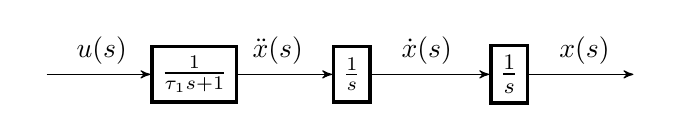
\begin{tikzpicture}[->,>=stealth',node distance=1.5cm]

	\node(vstup) {
 	};
 	
	\node[state, right of = vstup, shift = (right:0.5cm)] (kk2) {
  		$\frac{1}{\tau_1s + 1}$
 	};
 	
 	
	\node[state, right of = kk2, shift = (right:0.5cm)] (int1) {
  		$\frac{1}{s}$
 	};
 	
	\node[state, right of = int1, shift = (right:0.5cm)] (int2) {
  		\large{$\frac{1}{s}$}
 	};
 	
	\node[right of = int2, shift = (right:0.2cm)] (output) {
 	};

	\path (vstup.east)+(0.7cm, 0.3cm) node (label0) {\textbf{$u(s)$}};
	\path (kk2.east)+(0.5cm, 0.3cm) node (label1) {\textbf{$\ddot{x}(s)$}};
	\path (int1.east)+(0.7cm, 0.3cm) node (label3) {\textbf{$\dot{x}(s)$}};
	\path (int2.east)+(0.7cm, 0.3cm) node (label4) {\textbf{$x(s)$}};
       
	\path[->] (vstup) edge ($(kk2.west)$);
	\path[->] (kk2.east) edge ($(int1.west)$);
	\path[->] (int1.east) edge ($(int2.west)$);
	\path[->] (int2.east) edge (output);

\end{tikzpicture}
\caption{Diagram of the continuous system.}
\label{fig:LTI}
\end{figure}

The input action $u(s)$, as a from the MPC, is given to the KK2 and transformed to the the UAV's tilt, which corresponds to the real acceleration $\ddot{x}(s)$, and then twice integrated to the position ${x}(s)$.

\subsection{Coordinate systems}
\label{ssec:coordinate_system}
This whole thesis will consider 2D coordinate system only. In these 2 dimensions, there is an aileron axis $x$ with the direction to the right and the elevator axis $y$ with the direction forwards. These both axes are perpendicular. There are two coordinate systems which will be used. The first system is a standard world coordinate system W with the origin usually at the starting point of the UAV. The second system is a coordinate system U, which is a system with the origin in the center of the mass of the UAV. This is for example the coordinate system of detecting obstacles, which are observed relatively to the UAV by on-board cameras. Coordinate system U is created only by the translation of the system W by the vector $\vec{r} = (\Delta x, \Delta y)$. There is no rotation between the two coordinate systems, so the axes of the both coordinate systems are parallel. Because the UAV can move easily along each axis, there is no need to introduce the UAV's rotation. If the UAV rotated over time, the model would no longer be linear and the control of this system would be much more complex, therefore slower. These coordinate systems transformations follow equations

\begin{equation}
\label{eq:coordinate_transform}
\begin{split}
x^{(W)} &= x^{(U)}+\Delta x	\\
y^{(W)} &= y^{(U)}+\Delta y	\\
\dot{x}^{(W)} &= \dot{x}^{(U)}+\Delta \dot{x}	\\
\dot{y}^{(W)} &= \dot{y}^{(U)}+\Delta \dot{y}	\\
\ddot{x}^{(W)} &= \ddot{x}^{(U)}+\Delta \ddot{x}	\\
\ddot{y}^{(W)} &= \ddot{y}^{(U)}+\Delta \ddot{y}.	\\
\end{split}
\end{equation}
In the following text the world coordination system W will be used unless stated otherwise. The UAV has its own proportions. However, it is complicated to take into consideration the whole UAV's body. It is easier to proximate the UAV's body with a single mass point in its center. The orientation of the UAV is constant and will not be taken into consideration, thus the position of the UAV can be described by two coordinates. 

The altitude of the UAV is controlled separately. There are several reasons to do that. The first reason is, that many applications treat the altitude differently and enforce constant altitude for long periods of time. For example, in building interiors, the altitude is constant most of the time. The desired trajectory is also usually given in 2D and the altitude is described separately. The second reason is, as mentioned above, an MPC is very demanding on computing time. To save computational capacity, a standard PID controller can be used instead of an MPC for controlling the altitude. The altitude PID controller has already been implemented \cite{tomas} and it is not a part of this thesis. 

\subsection{State observer}
\label{sec:state_observer}
An MPC is very sensitive to a data noise and errors. Inaccurate initial condition can result in a bad prediction because of the double integration of acceleration into position. To work properly, the MPC requires very accurate initial conditions. These are position, speed and acceleration in both axes. A Kalman estimator has been implemented\cite{tomas} to estimate states of the UAV and disturbances of the acceleration. The inputs of the state observer are the system's input action and measured speed by a camera sensor.

%% Hovd, Morten. "A brief introduction to Model Predictive Control." URL= http://www. itk. ntnu. no/fag/TTK4135/viktig/MPCkompendium% 20HOvd. pdf (2004).


\subsection{Single axis model}
% picture of UAV
The UAV model has been analyzed\cite{tomas}. Thanks to the symmetrical body of the UAV, both axes share the same model. For aileron axis, the states take form of $\vec{x}_x = (x_x, \dot{x}_x, \ddot{x}_x)^T$ and $\vec{x}_y = (x_y, \dot{x}_y, \ddot{x}_y)^T$ for elevator axis, where $x_x$ is the aileron and $x_y$ is the elevator position. The aileron and elevator models are mathematically identical. The discrete state space model takes form of system matrices $\textbf{A}_s, \textbf{B}_s$ as

\begin{equation}
\label{eq:state_space_model_simple}
\vec{x}_{x,y,[t+1]} = \textbf{A}_{s} \vec{x}_{x,y, [t]} +\textbf{B}_{s} u_{x,y, [t]},
\end{equation} 
where $u_{x,y,[t]}$ is an input at time $t$, sampling with the frequency of $1/\Delta t = 70\jed{Hz}$.

\begin{equation}
\textbf{A}_{s} =
  \begin{bmatrix}
  1 & \Delta t & 		0 \\
  0 & 		 1 & \Delta t \\
  0	& 		 0 &		p_1
  \end{bmatrix},\textbf{B}_{s} = \begin{bmatrix}
  0 \\
  0 \\
  p_2
  \end{bmatrix}, 
\end{equation}
where $p_1 = 0.9799$ and $p_2 = 5.0719\cdot10^{-5}$. The unconstrained MPC can be solved separately for elevator and aileron axis. Simple constraints, such as input saturation can be applied.

\section{Model predictive control formulation}
\label{sec:Model_predictive_control_formulation}

An MPC is an advanced regulator. It uses prediction of future states of a system to determine system input actions. This prediction runs constantly in a loop. Because of its computational demands, it is used mainly in processes with long time constants. A motivation for its development was to control various chemical processes, where the computational time was not limiting. Using an MPC for controlling a UAV is a challenge, because it is hard to implement on embedded hardware. Controlling a real time system, such as UAV, requires regulation in tens of Hz, giving the hardware very little time to compute such a complex problem.

An MPC requires the system's state space model, initial condition and, unlike other controllers, a sequence of desired future states. An advantage of an MPC is applying large variety of constraints, which can be useful for example in the of chemical processes control. On the other hand, an MPC is sensitive to the model's inaccuracy and to sensory noise. 

Output of an MPC is not only the desired input action for the next time step, but also predicted input actions and predicted behavior of the system in the whole prediction horizon for the T following time steps. Unlike standard controllers like a PID, an MPC can adjust the input action based on future demands.

The MPC controller for tracking desired trajectory was developed \cite{tomas}. The goal of the thesis is to extend the controller to be capable of obstacle avoidance by using linearly constrained quadratic optimization. Obstacles are not previously known and can change position.

The MPC formulates optimization problem, that then has to be solved. The problem takes usually form of Linear Programming (LP) or, in this case, Quadratic Programming (QP).



\subsection{Extended model}		% extended?
For complex MPC constraints, such as position constraints for obstacle avoidance, position of UAV in one axis is a function of the position in the other axis. For these kinds of constraints axes can not be treated separately and more complicated system description is needed. The state space system must be preserved, connecting both identical systems for each axis into one system extending Eq. (\ref{eq:state_space_model_simple}) into 

\begin{equation}
\label{eq:state_space_model_simple}
\textbf{x}_{[t+1]} = \textbf{A} \textbf{x}_{[t]} +\textbf{B} \textbf{u}_{[t]},
\end{equation}
where $\textbf{u}_{[t]} = (u_{x,[t]}, u_{y,[t]})^T$ is an input vector containing elevator and aileron system inputs at the time $t$. Extended state vector 
\begin{equation}
\textbf{x}_{[t]} = (x_{[t]}, \dot{x}_{[t]}, \ddot{x}_{[t]}, y_{[t]}, \dot{y}_{[t]}, \ddot{y}_{[t]})^T
\end{equation}
contains positions $x,y$ and their derivatives at the time $t$. 

By connecting these two single axis systems, we get the following state space matrices of the extended system
\begin{equation}
\label{eq:state_space}
\textbf{A} = \begin{bmatrix}
	\textbf{A}_s & \textbf{0}	\\
	\textbf{0}   & \textbf{A}_s
\end{bmatrix}, \textbf{B} = \begin{bmatrix}
	\textbf{B}_s & \textbf{0}	\\
	\textbf{0}   & \textbf{B}_s
\end{bmatrix}.
\end{equation}






% graphs of saturated controllers:
%		1) MPC with only saturated inputs
%		2) MPC with saturated outputs
%		3) PID with saturated outputs



\subsection{System prediction}
The MPC algorithm is based on predicting future states based on initial condition and system input. Such a general equation can be derived from the Eq. (\ref{eq:state_space_model_simple}). With a simple substitution we can get prediction of the states at the time $t = 2$:

\begin{equation}
\begin{split}
\label{eq:mpc_lti_system2}
\textbf{x}_{[1]} &= \textbf{A}\textbf{x}_{[0]} + \textbf{B}\textbf{u}_{[0]},\\
\textbf{x}_{[2]} &= \textbf{A}\textbf{x}_{[1]} + \textbf{B}\textbf{u}_{[1]}\\
&= \textbf{A}\cdot(\textbf{A}\textbf{x}_{[0]} + \textbf{B}\textbf{u}_{[0]}) + \textbf{B}\textbf{u}_{[1]} \\
&=\textbf{A}^2\textbf{x}_{[0]} + \textbf{A}\textbf{B}\textbf{u}_{[0]} + \textbf{B} \textbf{u}_{[1]}.
\end{split}
\end{equation}
The Eq. (\ref{eq:mpc_lti_system2}) can be rewritten in a more general way:

\begin{equation}
\label{eq:mpc_lti_system_general}
\textbf{x}_{[t]} =\textbf{A}^t\textbf{x}_{[0]} + 
\sum_{i = 1}^{t-1}\textbf{A}^{i}\textbf{B}\textbf{u}_{[i-1]} + \textbf{B} \textbf{u}_{[0]}.
\end{equation}

Let's combine the sequence of the predicted states into a column vector
\begin{equation}
\textbf{\underline{x}} = (\textbf{x}_{[1]}^T, \textbf{x}_{[2]}^T, ..., \textbf{x}_{[T]}^T)^T
\end{equation}
of the length $6T$ and the sequence of the inputs into a column vector
\begin{equation}
\uvec = (\textbf{u}_{x,[0]}, \textbf{u}_{y,[0]}, \textbf{u}_{x,[1]}, \textbf{u}_{y,[1]}, ..., \textbf{u}_{x,[T-1]}, \textbf{u}_{y,[T-1]})^T.
\end{equation}
of the size $2T$. With this notation, Eq. (\ref{eq:mpc_lti_system_general}) can be represented as a matrix multiplication equation

\begin{equation}
\label{eq:prediction_big}
\underbrace{
\begin{bmatrix}
\textbf{x}_{[1]} \\
\textbf{x}_{[2]} \\
\vdots \\
\textbf{x}_{[T]} \\
\end{bmatrix}}_{\textbf{\underline{x}}}
=
\underbrace{
\begin{bmatrix}
\textbf{A} \\
\textbf{A}^2 \\
\vdots \\
\textbf{A}^{(T-1)} \\
\end{bmatrix}}_{\textbf{\^A}}
\textbf{x}_{[0]}
+
\underbrace{
\begin{bmatrix}
\textbf{B} & \textbf{0} & \textbf{0} & \textbf{0} \\
\textbf{AB} & \textbf{B} & \textbf{0} & \textbf{0} \\
\vdots & \vdots & \ddots & \vdots \\
\textbf{A}^{(T-1)}\textbf{B} & \textbf{A}^{(T-2)}\textbf{B} & \hdots & \textbf{B}
\end{bmatrix}
}_{\textbf{\^B}}
\cdot
\underbrace{
\begin{bmatrix}
\textbf{u}_{[0]} \\
\textbf{u}_{[1]} \\
\vdots \\
\textbf{u}_{[T-1]} \\
\end{bmatrix}}_{\uvec}.
\end{equation}
Using this new notation, Eq. \ref{eq:prediction_big} can be rewritten in a simpler form as

\begin{equation}
\label{eq:prediction_final}
\textbf{\underline{x}} = \textbf{\^A}\textbf{x}_{[0]} + \textbf{\^B}\uvec.
\end{equation}

\section{MPC implementation}
As mentioned in the Sec. \ref{sec:Model_predictive_control_formulation}, MPC formulates a quadratic optimization problem. This problem can be either constrained or unconstrained, depending on if constraints are demanded. Let's first solve the problem, where the obstacles are not involved. 
\subsection{Trajectory}
For MPC to compute input actions, there must be given a desired trajectory $\textbf{\underline{x}}_d = 
(\textbf{x}_{d,[1]}^T, \textbf{x}_{d,[2]}^T, ..., \textbf{x}_{d,[T]}^T)^T$, where the desired state at the time $t$ is $\textbf{x}_{d,[t]} = (x_{d,[t]}, \dot{x}_{d,[t]}, \ddot{x}_{d,[t]}, y_{d,[t]}, \dot{y}_{d,[t]}, \ddot{y}_{d,[t]})^T$. These desired states contain, besides aileron and elevator position, also velocity and acceleration. This gives the MPC a chance to  enforce other properties besides position. However, The UAV desired velocity is already given by the desired positions at certain time as the distance 

\begin{equation}
d = \sqrt{(x_{d,[t]}-x_{d,[t+1]})^2+ (y_{d,[t]}- y_{d,[t+1]})^2}.
\end{equation} 
The same method can be applied for acceleration. Therefore, the velocity and acceleration are demanded in the sequence of desired positions, rather than the desired system states. The desired velocity and acceleration are then ignored and it can hold any value, for example 0. The $\textbf{x}_{d,[t]}$ then takes form of $\textbf{x}_{d,[t]} = (x_{d,[t]}, 0, 0, y_{d,[t]}, 0, 0)^T$. When creating the desired trajectory, one must always keep in mind, that the desired positions hold also information about velocity and acceleration.

\subsection{Objective function}
\label{sec:objective_function}
As in many other areas of engineering, the problem can be split into two independent parts. Creating an objective function and then minimizing it. The objective function's (sometimes called a cost function) value describes, how good is the particular solution. The set of particular solutions is the domain of the objective function. In this case the solution takes form of a vector $\underline{\textbf{u}}$, which can be directly transformed into predicted trajectory. The lower the value of the objective function is, the better is the particular solution. The solution with the minimal objective function's value is called an optimal solution.

The goal of unconstrained MPC is to track a given trajectory as well as possible. This means, that we want to minimize the distance between all the predicted and the desired positions. This error in both axes can be computed as
\begin{equation}
\begin{split}
\label{eq:simple_err}
e_{x, t} &= x_{[t]} - x_{d, [t]}\\
e_{y, t} &= y_{[t]} - y_{d, [t]}.
\end{split}
\end{equation}
Using this kind of error has many downsides. The obvious one is, that it penalizes error in only one direction and favors the other. If we want to use the distance, we would have to take the absolute value. This function would not be differentiable \cite{stein1970singular} and solving this task would be more complicated. Differentiability is a very useful property. Being able to compute gradient of the final objective function results in fast task solving. Above that we don't get very good results if penalizing the error linearly. 

From the experience, it has come beneficial in many ways to use the the the square of the error. This preserves the condition of not prioritizing one direction error. The function is also easily differentiable. The next great advantage is penalizing big distances disproportionately more and ignoring very small errors. This also describes our requirements, where the exact tracking of the trajectory is not as important as eliminating big deviations from the trajectory. If a simple sum of $e_{x, t}^2$ and $e_{y, t}^2$ was applied, the system would behave very wildly, generating very high input actions to correct the error. However, this is not in the capabilities of the real system and could result in an unstable control. Therefore input actions must be also penalized. When combined together, we get the following objective function 

\begin{equation}
\label{eq:qmpc_basic_formulation}
% mala chyba, x nezahrnuje x0.
\mathrm{V}\left(\textbf{e}_x, \textbf{e}_y, \uvec\right) 
= \frac{1}{2}\sum_{i=1}^{T}\left( k_q \cdot (e^2_{x, [i]}+e^2_{y, [i]}) + k_s \cdot (\textbf{u}^2_{x, [i-1]}+\textbf{u}^2_{y, [i-1]})\right),
\end{equation}
where $\textbf{e}_x = (e_{x, [1]}, e_{x, [2]}, ..., e_{x, [T]})^T$ and $\textbf{e}_y = (e_{y, [1]}, e_{y, [2]}, ..., e_{y, [T]})^T$. The ratio of the constants $k_q$ and $k_s$ is the only parameter of the MPC and determines how wildly the system behaves. The error at the time $t = 0$ is determined only by the initial condition and doesn't depend on on the input action $\uvec$. Because the function is to be optimized, this error can be left out. The Eq. (\ref{eq:qmpc_basic_formulation}) can be rewritten in a matrix form using penalizing matrices $\textbf{Q}$ and $\textbf{S}$

\begin{equation}
\label{eq:qmpc_sum}
\mathrm{V}\left(\textbf{\underline{e}}, \uvec\right) = \frac{1}{2}\sum_{i=1}^{T}\left(\textbf{e}^T_{[i]}\textbf{Q}\textbf{e}_{[i]} + \textbf{u}^T_{[i-1]}\textbf{P}\textbf{u}_{[i-1]}\right),
\end{equation}
where $\underline{\textbf{e}} = \underline{\textbf{x}} - \underline{\textbf{x}}_d$ is the error of all states at the time $t$  and matrices $\textbf{Q}$ and $\textbf{P}$ are

\begin{equation}
\label{eq:qmpc_weighting_matrices_simple}
\textbf{Q} = \begin{bmatrix}
k_q & 0 & 0 & 0 & 0 & 0 \\
0 & 0 & 0 & 0 & 0 & 0 \\
0 & 0 & 0 & 0 & 0 & 0 \\
0 & 0 & 0 & k_q & 0 & 0 \\
0 & 0 & 0 & 0 & 0 & 0 \\
0 & 0 & 0 & 0 & 0 & 0 \\
\end{bmatrix}, 
\textbf{P} = \begin{bmatrix}
k_p & 0\\
0 & k_p\\
\end{bmatrix}.
\end{equation}

This form of $\textbf{Q}$ allows to penalize only position errors and ignore the velocity and acceleration errors. For a fast optimization, the objective function has to be convex, as described in the section ---CONVEXITY???---. To ensure, that the function $\mathrm{V}\left(\textbf{\underline{x}}, \uvec\right)$ is strictly convex, the matrix $\textbf{Q}$ must be positive semi-definite ($\textbf{Q} \succeq 0$) and $\textbf{P}$ must be positive definite ($\textbf{P} \succ 0$). The matrix $\textbf{Q}$ has it's eigenvalues $0$ and $k_q$, therefore $k_q \geq 0$. The eigenvalues of $\textbf{P}$ are $k_p$, so $k_p > 0$. In some MPC algorithms the last error is penalized with higher weight, forcing the system to end up in the last state more. It turned out, this can be counterproductive in obstacle avoidance system for reasons that will be discussed later.

We want to get rid of the sum in Eq. (\ref{eq:qmpc_sum}) and substitute it with matrix multiplication. Let's first introduce the matrices $\textbf{\^Q}$ and $\textbf{\^P}$ as 

\begin{equation}
\label{eq:qmpc_weighting_matrices}
\textbf{\^Q} = \begin{bmatrix}
\textbf{Q} & \textbf{0} & \hdots & \textbf{0} \\
\textbf{0} & \textbf{Q} & \hdots & \vdots \\
\textbf{0} & \hdots & \ddots & \vdots \\
\textbf{0} & \hdots & \hdots & \textbf{Q}
\end{bmatrix},
\textbf{\^P} = \begin{bmatrix}
\textbf{P} & \textbf{0} & \hdots & \textbf{0} \\
\textbf{0} & \textbf{P} & \hdots & \vdots \\
\textbf{0} & \hdots & \ddots & \vdots \\
\textbf{0} & \hdots & \hdots & \textbf{P}
\end{bmatrix}.
\end{equation}

If the last error was to be penalized more, the last matrix $\textbf{Q}$ on the diagonal of the matrix $\textbf{\^Q}$ would consist of higher constants $k_q$. Lets rewrite the Eq. (\ref{eq:qmpc_sum}) using the Eq. (\ref{eq:prediction_final}):

\begin{equation}
\begin{split}
\label{eq:qmpc_counting}
\mathrm{J}(\underline{\textbf{u}}) 
&= \frac{1}{2}\bigg(\underline{\textbf{e}}^T 
\textbf{\^Q} \underline{\textbf{e}}+\underline{\textbf{u}}^T 
\textbf{\^P} \underline{\textbf{u}}\bigg)\\
&=\frac{1}{2}\bigg((\textbf{\^A}\textbf{x}_{[0]} + \textbf{\^B}	  \uvec-\underline{\textbf{\~x}})^T 
\textbf{\^Q}
(\textbf{\^A}\textbf{x}_{[0]} + \textbf{\^B}\uvec-\underline{\textbf{\~x}}) 
+\underline{\textbf{u}}^T 
\textbf{\^P} \underline{\textbf{u}}\bigg)\\
&=\frac{1}{2}\bigg(
2(\textbf{\^Q}\textbf{\^B})^T \textbf{\^A} \textbf{x}_{[0]} \underline{\textbf{u}}
+\uvec^T \textbf{\^B}^T\textbf{\^Q} \textbf{\^B}\uvec
-2(\textbf{\^Q}\textbf{\^B})^T \underline{\textbf{\~x}}\; \underline{\textbf{u}}
+\underline{\textbf{u}}^T 
\textbf{\^P} \underline{\textbf{u}}+const.\bigg)
\end{split}
\end{equation}

In the Eq. (\ref{eq:qmpc_counting}), all constant elements have been put into the $const$ part. Because the goal is to minimize the objective function $\mathrm{J}(\underline{\textbf{u}})$, parts of the equation, that do not depend on the $\underline{\textbf{u}}$ can be left out. The Eq. (\ref{eq:qmpc_counting}) can be rewritten as

\begin{equation}
\mathrm{J}(\underline{\textbf{u}}) = \frac{1}{2}\uvec^T\underbrace{\left(\textbf{\^B}^T\textbf{\^Q}\textbf{\^B} + \textbf{\^P}\right)}_{\textbf{\^H}}\uvec + \underbrace{\left(\textbf{\^Q}\textbf{\^B}\right)^T\left(\textbf{\^A}\textbf{x}_{[0]} - \textbf{\underline{\~x}}\right)}_{\textbf{\^c}}\uvec.
\label{eq:mpc_objective_large}
\end{equation}

The task can be formulated as

\begin{equation}
\label{eq:qmpc_main_quadratic_form}
\begin{aligned}
& \min_{\uvec \in \mathrm{R}^{kM}}
& & \mathrm{J}(\uvec) = \frac{1}{2}\uvec^T\textbf{\^H}\uvec + \textbf{\^c} \uvec\\
& \text{s.t.}
& & \textbf{A}_c \uvec \leq \textbf{B}_c.
\end{aligned}
\end{equation}
The constraints will be further discussed in section \ref{sec:system_constraints}. For unconstrained system we can ignore them.

\subsection{Solving QP unconstrained}
We want to solve the problem formulated in the Eq. \ref{eq:qmpc_main_quadratic_form} while ignoring the constraints. For this task to have a single optimal solution $\underline{\textbf{u}}^{\star}$, the objective function has to be convex. Therefore the matrix $\textbf{\^H}$ has to be positive semi definite. This is guaranteed, because the matrices  $\textbf{Q}$ and $\textbf{S}$ were chosen to be positive semi-definite ($\textbf{Q}, \textbf{S} \succeq 0$) and $\textbf{P}$ positive definite ($\textbf{P} \succ 0$). For solving this task, we need the gradient of the objective function \cite{zometa2012implementation} as
\begin{equation}
\label{eq:J_grad}
\nabla\macJ = \textbf{\^H}\uvec + \textbf{\^c}.
\end{equation}
The gradient $\nabla\mathrm{J}(\underline{\textbf{u}}) \in R^{2T}$ is a vector with the opposite direction to the global minimum, so the $-\nabla\mathrm{J}(\underline{\textbf{u}})$ is a vector pointing the direction towards the global minimum $\underline{\textbf{u}}^{\star}$. For solving this task, a gradient descent algorithm can be used, but also analytic solution can be found.  

Because the  $\textbf{\^H}$ is positive semidefinite, the quadratic form $\frac{1}{2}\uvec^T\textbf{\^H}\uvec$ is convex. The term $\textbf{\^c} \uvec$ is a linear function and adding it to a convex function does not change the convexity of the task. Because of this, we know, that a local minimum is also a global minimum. The local minimum can be found as 
\begin{equation}
\label{eq:J_local_min}
\begin{split}
\nabla\mathrm{J}(\underline{\textbf{u}}^{\star}) = \textbf{\^H}\underline{\textbf{u}}^{\star} + \textbf{\^c} &= 0 \\
\textbf{\^H}\underline{\textbf{u}}^{\star} &= - \textbf{\^c} \\
\underline{\textbf{u}}^{\star} &= -\textbf{\^H}^{-1}\textbf{\^c}.
\end{split}
\end{equation}
The inverse of $\textbf{\^H}$ can be computed, because $\textbf{\^H}$ is positive-definite, therefore regular. This is guaranteed by the definition of positive-definite property, that its leading principal minors are all positive \cite{chong2013introduction}. On-board computation is fast, because matrix $\textbf{\^H}^{-1}$ does not depend on the system state and is only the function of the constants $k_q$, $k_p$ and the system model. It can be generated in advance and stored as a constant in the UAV's read-only memory. Finding the $\underline{\textbf{u}}^{\star}$ is only matter of creating vector $\textbf{\^c}$ and computing $-\textbf{\^H}^{-1}\textbf{\^c}$.


\subsection{System constraints} \label{sec:system_constraints}
One of the greatest advantages of MPC is being able to apply large variety of constraints. As mentioned in section \ref{eq:QP_formulation}, the MPC uses linearly constraint quadratic programming for finding the input action prediction. There can be many different kinds of constraints and the MPC has to obey all of them. These constraints take form of linear inequalities

\begin{equation}
\label{eq:constraint_ineq_simple}
\macoi \cdot \uvec \leq b_i, \;\;\; i \in \{1, 2, ..., m\},
\end{equation}
where $\vec{\omega}_i$ is a vector of the length 2T and $b_i$ is a scalar, both describing the constraint number $i$. $m$ is the total number of constraints applied. Each constraint takes form of a half space in in a space $\textbf{R}^{2T}$ constraining it by hyperplane with a normal vector $\vec{\omega}_i$ shifted by $b_i$. To apply multiple constraints at the same time, the Eq. (\ref{eq:constraint_ineq_simple}) can be rewritten in matrix form as 

\begin{equation}
\label{eq:MPC_cond}
\textbf{A}_c \uvec \leq \textbf{B}_c,
\end{equation}
where $\textbf{A}_c$ is a matrix of the width 2T and height $m$ - the number of constraints applied. $\textbf{B}_c$ is a column vector of the same height created as

\begin{equation}
\textbf{A}_c =
  \begin{bmatrix}
  \vec{\omega}_1 \\
  \vec{\omega}_2 \\
  ...	   \\
  \vec{\omega}_m
  \end{bmatrix},\textbf{B}_c = \begin{bmatrix}
  b_1 \\
  b_2 \\
  ... \\
  b_m
  \end{bmatrix}.
\end{equation}
Each line of the matrix $\textbf{A}_c$ together with a particular member of $\textbf{B}_c$ represents one constraint. 

\subsection{Input constraints}
\label{sec:input_constraints}
\begin{figure}[h]
%% edit second figure to predicted action saturated
\centering
\begin{subfigure}[b]{0.5\textwidth}
	\includegraphics[width=\textwidth]{fig/step_constrained_2.eps}
	\caption{constrained MPC.}
	\label{fig:mpc_constrained}
\end{subfigure}%
\begin{subfigure}[b]{0.5\textwidth}
	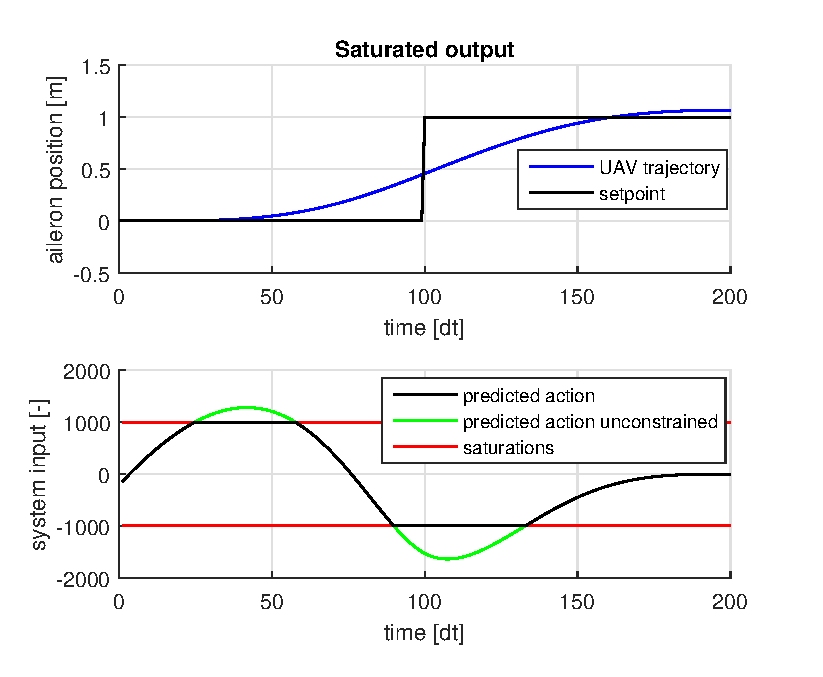
\includegraphics[width=\textwidth]{fig/step_saturated_2.eps}
	\caption{saturated MPC.}
	\label{fig:mpc_saturated}
\end{subfigure}
\caption{Step response of the system using two approaches of saturation.}
\end{figure}

In control engeneering, a common problem one must overcome is a system saturation. This means, that the real system is linear only on a certain range of inputs and has limited capapibilities \cite{saturation}. For example motor can spin in a certain maximum speed despite input voltage. If the system receives too high input actions from the controller, it can get damaged. This can happen for example in PD control, when the difference between real and desired output changes rapidly in time, for example because of a sensory noise.
A standard  solution for this problem is a simple saturation of the output of the controller. This is a simple solution and for many tasks it is enough. However, because the controller doesn't take into consideration this saturation, the system can behave incorrectly.
The advantage of MPC is, that the controller can consider these aspects of real system and find an input prediction, that will not violate the constraints and at the same time will achieve the desired output. This is achieved by the MPC constraints. The system saturation thresholds are $u_{min}$ and $u_{max}$. We can see in fig. (\ref{fig:mpc_saturated}) simply saturated input action with the computed trajectory and int fig. (\ref{fig:mpc_constrained}) the input action computed by the MPC using system constraints. 

\section{Collision Avoidance}
Collision avoidance in MPC is realized through constraining the position. This means, that we allow every predicted position to be in a certain allowed space and every violation of this space is considered to be a collision. For the UAV to get outside this allowed space will be prohibited by the algorithm used in this section. In the subsection \ref{ssec:coordinate_system} has been introduced, that the UAV is approximated with a single point of mass. Using this approximation would result only for the center point of the UAV not to collide. In the real world the size matters. it is not necessary to bring the whole model back. Instead the whole body can be approximated with a ring with the same center $(x, y)$ and radius $R$, such as every part of the body $(x_b, y_b)$ follows $|x - x_b, y - y_b| \leq R$. If the distance between the position of UAV and the edge of the allowed space is less or equal $R$, it can be said, that the UAV will not collide. 

The biggest problem in using MPC as a collision avoidance is creating this allowed space and converting it to the MPC constraints. 

\subsection{Convexity}
\label{sec:convexity}
Let's start with the definition of convexity. A set $S$ is convex if
\begin{equation}
\label{eq:convexity_definition}
\forall\{x_1, x_2\} \in S, \forall t \in  \textless 0, 1 \textgreater \implies t \cdot x_1 + (1-t) \cdot x_2 \in S.
\end{equation}
In simple worlds, if every 2 points of a set are connected with a line, the whole line has to belong to the set.

For easily finding the global minimum of the cost function $\mathrm{J}(\underline{\textbf{u}})$, it is essential to keep the problem convex. This has many levels. First we have to ensure, that the function J is convex. This has been discussed in Sec. \ref{sec:objective_function}. Lets introduce a space $S$ of dimension $2T+1$, where the axes will be $(\uvec^T, z)$. Then introduce a subset $J_s$ of the space $S$ as $\{J_s \in S : \mathrm{J}(\underline{\textbf{u}}) \leq z\}$. The function $\mathrm{J}(\underline{\textbf{u}})$ is convex, if and only if the subset $J_s$ is convex. 
\subsubsection{Convexity of u}
Lets have a look at the vector $\underline{\textbf{u}}$. For MPC purposes this vector is is needed to be constrained. Because the space $S$ has one more dimension than $\underline{\textbf{u}}$, an extended version will be needed such as $(\underline{\textbf{u}}^T, z)^T$.
All points, that satisfy the condition \ref{eq:MPC_cond} will create a subset $U_s$ such as $\{U_s \in S : \textbf{A}_c \cdot \underline{\textbf{u}} \leq \textbf{B}_c\}$. The condition is independent of $z$, so it is defined for all $z$. 

We can look at this as the feasible $\underline{\textbf{u}}$ is the domain of the function $\mathrm{J}(\underline{\textbf{u}})$. Let's examine, how the $U_s$ actually looks. As mentioned in the Sec. \ref{sec:system_constraints}, the feasible $\underline{\textbf{u}}$ is an $\underline{\textbf{u}}$, that satisfies $m$ linear inequalities represented as half spaces. To satisfy all of them, set $U_s$ has to be an extended intersection of half spaces. This is important, because the convexity of set $U_s$ can be now proven. 

\subsubsection{Proof of the convexity of polytope}

A theorem states, that an intersection of convex sets creates a convex set. An intersection of finite number of half spaces is a convex polytope. This polytope doesn't have to be bounded. Such a polytope is shown on a figure \ref{fig:convex_polytope} in only 2 dimensions constrained by 3 half spaces.

\begin{figure}[h]
\centering
\includegraphics[width=0.7\textwidth]{fig/convex_polytope.eps} 
\caption{convex polytope.}
\label{fig:convex_polytope}
\end{figure}

At this time is left to prove, that a single half space is a convex set. Half space is described in Eq. (\ref{eq:constraint_ineq_simple}) as $\{\uvec : \omega_i \cdot \uvec \leq b_i$ for $i \in \{1, 2, ..., m\}\}$. If we take any 2 points $\uvec_1, \uvec_2$ belonging to the half space given by the normal vector $\omega_i$ and bias $b_i$, the line segment between them has to lie in the half space. This can be proved for any dimension. The line segment is described as

\begin{equation}
\label{eq:convex_line}
t \cdot \uvec_1 + (1-t) \cdot \uvec_2; \;\;\; t \in \textless 0, 1 \textgreater
\end{equation}

The problem of proving convexity has been transformed using the Eq. (\ref{eq:convex_line}) into equation 

\begin{equation}
\label{eq:convex_u_proof}
\omega_i \cdot (t \cdot \uvec_1 + (1-t) \cdot \uvec_2) \leq b_i.
\end{equation}
We know, that $\uvec_1$ and $\uvec_2$ belong to the half space, therefore 
\begin{equation}
\begin{split}
\omega_i \cdot \uvec_1 &\leq b_i\\
\omega_i \cdot \uvec_2 &\leq b_i.
\end{split}
\end{equation}

Because $\omega_i \cdot \uvec$ is a scalar, there are just 3 possible outcomes. $\omega_i \cdot \uvec_1 = \omega_i \cdot \uvec_2$ or $\omega_i \cdot \uvec_1 < \omega_i \cdot \uvec_2$ or $\omega_i \cdot \uvec_1 > \omega_i \cdot \uvec_2$. Lets have a look at the first case $\omega_i \cdot \uvec_1 = \omega_i \cdot \uvec_2:$


\begin{equation}
\begin{split}
\omega_i \cdot (t \cdot \uvec_1 + (1-t) \cdot \uvec_2) &\leq b_i\\
\omega_i \cdot (\uvec_1(t+1-t) &\leq b_i\\
\omega_i \cdot \uvec_1 &\leq b_i.
\end{split}
\end{equation}
This case has been proven. The second case $\omega_i \cdot \uvec_1 < \omega_i \cdot \uvec_2$ is a little bit more complicated. Because $\omega_i \cdot \uvec_2 \leq b_i.$ It would be sufficient to prove 

\begin{equation}
\label{eq:conv_proof_1_less_2}
\begin{split}
\omega_i(t \cdot \uvec_1 + (1-t) \cdot \uvec_2) &\leq \omega_i \cdot \uvec_2\\
\omega_i(t \cdot \uvec_1 -t \cdot \uvec_2) &\leq 0\\
t \cdot \omega_i(\uvec_1 - \uvec_2) &\leq 0\\
\omega_i \cdot \uvec_1 &\leq \omega_i \cdot \uvec_2.
\end{split}
\end{equation}
The third line has been divided by $t$. In case $t = 0$, the proof ends by $0 \leq 0$, otherwise continuing to the fourth line. This case has been also proven. Proving the last case $\omega_i \cdot \uvec_2 < \omega_i \cdot \uvec_1$ is very similar. 

\begin{equation}
\label{eq:conv_proof_2_less_1}
\begin{split}
\omega_i(t \cdot \uvec_1 + (1-t) \cdot \uvec_2) &\leq \omega_i \cdot \uvec_1\\
\omega_i((t - 1) \cdot \uvec_1 - (t - 1) \cdot \uvec_2) &\leq 0 \\
(t - 1) \cdot \omega_i \cdot (\uvec_1 - \uvec_2) &\leq 0 \\
\omega_i \cdot \uvec_1 &\leq \omega_i \cdot \uvec_2
\end{split}
\end{equation}

Similarly to the Eq. (\ref{eq:conv_proof_1_less_2}), the third line of the Eq. (\ref{eq:conv_proof_2_less_1}) has been divided by $t-1$. 
It has been proven, that all $\uvec$, that obey the Eq. (\ref{eq:MPC_cond} c)reate a convex set. This means, that also the set $U_s$ is convex. Intersection of the convex set $J_s$ and $U_s$ is a convex set making the function $\mathrm{J}(\underline{\textbf{u}})$ with the domain as polytope defined $\textbf{A}_c \uvec \leq \textbf{B}_c$ is a convex function.

\section{Obstacles}
Through this thesis, obstacles are represented by circles in 2D only. They have 3 parameters: position $x_{obs}$, position $y_{obs}$ and diameter $r_{obs}$. Despite obstacles can have various shapes, we simplify them to allow simpler computations. Because the MPC runs constantly in the loop and reacts to the changing environment, it also works with moving objects. Until now, the UAV body has been approximated with one mass point without considering its real size. Since it would be difficult to calculate, whether the UAV's body has collided, we use Minkovski sum. Instead of computing with the real size of the UAV, the representation of all obstacles will change according to the UAV's size, creating a circle with the UAV's dimensions. This circle will have the smallest possible diameter $R_{UAV}$ while still wrapping the UAV as shown in the Fig. \ref{fig:UAV_dimensions}. 

\begin{figure}[h]
\centering
\begin{minipage}{.48\textwidth}
  \centering
  \includegraphics[width=1\linewidth]{fig/UAV_dimensions.eps}
  \caption{UAV dimensions}
  \label{fig:UAV_dimensions}
\end{minipage}%
\begin{minipage}{0.48\textwidth}
  \centering
  \includegraphics[width=1\linewidth]{fig/blob.png}
  \label{fig:blob}
  \captionof{figure}{Recognizable marker}
\end{minipage}
\end{figure}




Let's define a simplified representation of the UAV's body. It can be now said, that the UAV will not collide, if 
\begin{equation}
(x_{obs} - x)^2 + (y_{obs} - y)^2 \geq (R_{UAV} + r_{obs})^2.
\end{equation}
From now on we will compute with the UAV as a single mass point and every obstacle's diameter $r_{obs}$ substitute with the $r_{obs} + R_{UAV}$.	 

Let's make an assumption, that the UAV's trajectory is a line created by connecting all the predicted positions. This line has a zigzag shape. Because the UAV can not change vector of speed immediately, the real trajectory has to have a continuous first time derivative. Also because the second derivative(acceleration) of the UAV's position is a result of the UAV's pitch and roll, which also can not be changed immediately, the second derivative is also continuous. In short, the real trajectory intersects all the predicted positions, but there is a small deviation caused by the first and second derivatives of the real system. The real trajectory has to be smooth up to second derivative. To be able to approximate the real trajectory by the simplified zigzag trajectory, we need to make sure, that the predicted positions are far closer to each other, than the obstacles sizes. This is easy to achieve, because the time between the predicted positions is $\Delta t = 1/70s$, which with the maximum speed of 0.35\jed{ms^{-1}} is distance of 5\jed{mm}.

\begin{figure}[h]
\centering
\includegraphics[width=1\textwidth]{fig/perfect_collision_avoidance_arrow.eps} 
\caption{UAV avoidance in non-convex space.}
\label{fig:perfect_collision_avoidance}
\end{figure}

The forward approach would be to say, that every trajectory is feasible, if any predicted position does not collide with any obstacle. This approach would search for any trajectory in the allowed space. However if the obstacle is just a simple circle, the allowed space is non-convex as shown in Fig. \ref{fig:perfect_collision_avoidance}. As mentioned in Sec.  \ref{sec:convexity}, for keeping the quadratic programming convex, the allowed space for UAV has to be convex. This turned out to be the greatest disadvantage of using MPC for obstacle avoidance. 

This is also the reason, why greater penalization of the last state deviation is not desirable. The allowed space is not ideal and the prediction of the last position 

\subsection{Creating allowed space}


A convex allowed space for trajectory planning has to be created to approximate the real world situation. However, there can not be enough good convex representation, that is robust at the same time. The approach for creating a convex allowed space in this thesis is restricting any position in a half plain 'behind' any obstacle as shown in Fig. \ref{fig:half_plain}. Combining multiple obstacle constraints, this space becomes polytope defined by a set of half planes. These plains are in each MPC iteration updated by the relative positions of the obstacles. These positions continuously change due to the UAV's movement and the sensory noise. Let's first look at a situation with a single obstacle. 

\begin{figure}[h]
\centering
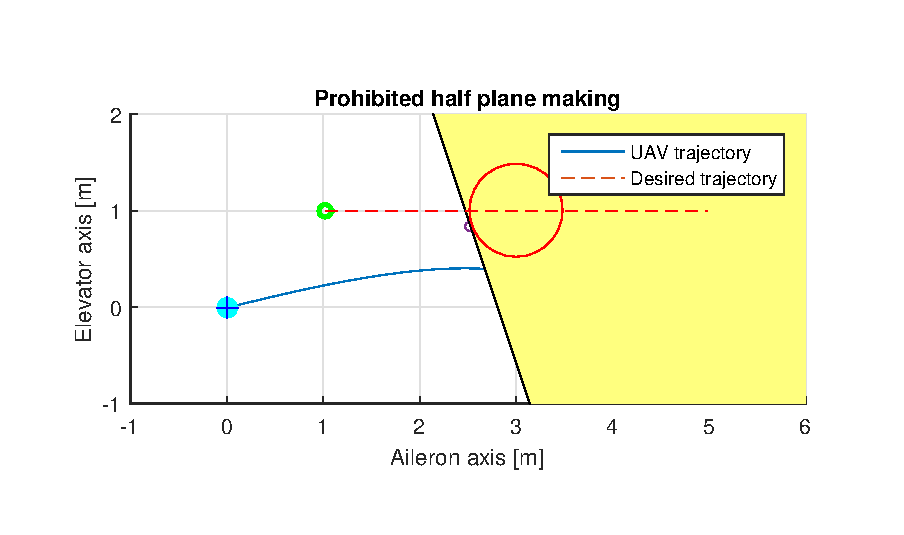
\includegraphics[width=1\textwidth]{fig/half_plain_making.eps} 
\caption{Creating a prohibited half plain}
\label{fig:half_plain}
\end{figure}

Half plane can be can be represented by the equation $y \leq kx + q$  where $x$ and $y$ are the allowed positions of UAV and $k$ is the slope of the line and $q$ is the bias of the line. For easier work, these equations can be rewritten as

\begin{equation}
\label{eq:simple_obstacle_cond}
s(y - kx - q) \leq 0,
\end{equation}
where $s = \pm 1$. This is an inequality defining one obstacle by a single half plain. 
These constants $k, q$ and $s$ can be found as 

\begin{equation}
\label{eq:obstacle_constants}
\begin{split}
k &= -\frac{y_{obs} - y_{UAV}}{x_{obs} - x_{UAV}}\\
b_x &= (x_{obs}-x_{UAV})\cdot \big(1-\frac{r_{obs}+R_{UAV}}{\sqrt{(x_{obs} - x)^2 + (y_{obs} - y)^2}} \big)\\
b_y &= (y_{obs}-y_{UAV})\cdot \big(1-\frac{r_{obs}+R_{UAV}}{\sqrt{(x_{obs} - x)^2 + (y_{obs} - y)^2}} \big)\\
q &= b_y - kb_x\\
s &= sign(y).
\end{split}
\end{equation}
The $b_x$ and $b_y$ is a position of the intersection of the constraining line and the obstacle circle with diameter $R_{UAV}+r_{obs}$. 

We have found the constrains for position. These constraints have to be further transformed into an input action constraints. This is an inverse transformation to the Eq. \ref{eq:prediction_final}, where input actions have been transformed to position and its derivatives. For the purposes of MPC, matrices $\textbf{A}_c $ and $\textbf{B}_c$ have to be created to fit the condition \ref{eq:MPC_cond}. The vector $\textbf{\underline{x}}$ from the Eq. \ref{eq:prediction_final} contains all predicted states for both axes. We are interested in separating just the predicted positions $x$ and $y$ into the position column vectors $\textbf{x}_p$ and $\textbf{y}_p$ of size $T$ as 

\begin{equation}
\textbf{x}_p =
  \begin{bmatrix}
  x_{[1]} \\
  x_{[2]} \\
  ...	   \\
  x_{[T]}
  \end{bmatrix},\textbf{y}_p = \begin{bmatrix}
  y_{[1]} \\
  y_{[2]} \\
  ...	   \\
  y_{[T]}
  \end{bmatrix},
\end{equation}
where $x_{[t]}$ is the predicted position $x$ at the time $t$ and $y_{[t]}$ is the predicted position $y$ at the time $t$.
These vectors are related to $\uvec$ by the matrices $\textbf{\^A}_x$, $\textbf{\^B}_x$, $\textbf{\^A}_y$, $\textbf{\^B}_y$ as
\begin{equation}
\label{eq:pos_matrixes}
\begin{split}
\textbf{x}_p &= \textbf{\^A}_x \textbf{x}_{[0]} + \textbf{\^B}_x \uvec \\
\textbf{y}_p &= \textbf{\^A}_y \textbf{x}_{[0]} + \textbf{\^B}_y \uvec, \\
\end{split}
\end{equation}
where the matrices $\textbf{\^A}_x, \textbf{\^A}_y$ $\in R^{T \times 6}$ and $\textbf{\^B}_x, \textbf{\^B}_y$ $\in R^{T \times 2T}$ are submatrices of their corresponding matrices  $\textbf{\^A}$, $\textbf{\^B}$, $\textbf{\^A}$, $\textbf{\^B}$ as 

\begin{equation}
\begin{split}
\textbf{B}_x &= 
\begin{bmatrix}
\textbf{B}_{1, 1:2} & \textbf{0} & \textbf{0} & \textbf{0} \\
\textbf{A}_{1, 1:6}\textbf{B} & \textbf{B}_{1, 1:2} & \textbf{0} & \textbf{0} \\
\vdots & \vdots & \ddots & \vdots \\
\textbf{A}^{(T-1)}_{1, 1:6}\textbf{B} & \textbf{A}^{(T-2)}_{1, 1:6}\textbf{B} & \hdots & \textbf{B}_{1, 1:2}
\end{bmatrix}, 
\textbf{A}_x = 
\begin{bmatrix}
\textbf{A}_{1, 1:6} \\
\textbf{A}^2_{1, 1:6} \\
\vdots \\
\textbf{A}^{(T-1)}_{1, 1:6} \\
\end{bmatrix}, \\
\textbf{B}_y &= 
\begin{bmatrix}
\textbf{B}_{4, 1:2} & \textbf{0} & \textbf{0} & \textbf{0} \\
\textbf{A}_{4, 1:6}\textbf{B} & \textbf{B}_{4, 1:2} & \textbf{0} & \textbf{0} \\
\vdots & \vdots & \ddots & \vdots \\
\textbf{A}^{(T-1)}_{4, 1:6}\textbf{B} & \textbf{A}^{(T-2)}_{4, 1:6}\textbf{B} & \hdots & \textbf{B}_{4, 1:2}.
\end{bmatrix},
\textbf{A}_y = 
\begin{bmatrix}
\textbf{A}_{4, 1:6} \\
\textbf{A}^2_{4, 1:6} \\
\vdots \\
\textbf{A}^{(T-1)}_{4, 1:6}
\end{bmatrix}.
\end{split}
\end{equation}
$\textbf{A}_{i_1, i_2:i_3}$ is a matlab-like notation describing a submatrix of the matrix $\textbf{A}$ with the line $i_1$ and columns from $i_2$ to $i_3$. The Eq. (\ref{eq:simple_obstacle_cond}) is defined only for one position. These matrices are constant, so they can be computed in advance and stored in the read-only memory. It is important, that the UAV does not collide in any predicted position in the prediction horizon. Then this equation is rewritten in a vector form

\begin{equation}
\label{eq:vector_obstacle_cond}
s(\textbf{y}_p - k\textbf{x}_p - \textbf{q}) \leq 0,
\end{equation}
where $\textbf{q}$ is the column vector of the size $T$ and every member is $q$.
 After the substitution of Eq. (\ref{eq:pos_matrixes}) into Eq. (\ref{eq:vector_obstacle_cond}) we get
 
\begin{equation}
\begin{split}
s\big(\textbf{\^A}_y \textbf{x}_{[0]} + \textbf{\^B}_y \uvec - k(\textbf{\^A}_x \textbf{x}_{[0]} + \textbf{\^B}_x \uvec) - \textbf{q}\big) &\leq 0 \\
\underbrace{s\big(\textbf{\^B}_y-k\textbf{\^B}_x\big)}_{\textbf{\^A}_c} \uvec +
\underbrace{s\big(\textbf{\^A}_y \textbf{x}_{[0]} - k\textbf{\^A}_x \textbf{x}_{[0]} -k\textbf{q}\big)}_{\textbf{B}_c} &\leq 0.
\end{split}
\end{equation}
Until now, all the half planes of the obstacles have been computed from the relative position of the initial position of the UAV. This means, that for example the last predicted position will be still constrained by the position some time ago. However we don't know the last position, because it can be computed from the vector $\uvec$ that we are searching for. If an assumption is made, that the predicted trajectory is very similar to the one in the previous step, we can use the previous one. The MPC loop runs in tens of Hz and the UAV doesn't change its position very much in the one time step. This improvement is done by computing the previous trajectory using Eq. (\ref{eq:prediction_final}). Then the constants $k_{i}, q_{i}, s_{i}$ need to be found for each predicted position $i, i\in\{1,...,T\}$ using the Eq. (\ref{eq:obstacle_constants}). Then the Eq. (\ref{eq:vector_obstacle_cond}) can be rewritten in a matrix form as

\begin{equation}
\label{eq:matrix_obstacle_cond}
\textbf{\^s}(\textbf{y}_p - \textbf{\^k}\textbf{x}_p - \textbf{q}) \leq 0,
\end{equation}
where $\textbf{\^s}$ and $\textbf{\^k}$ are square diagonal matrices of the size $T$.
\begin{equation}
\label{eq:obstacle_constants_matrices}
\textbf{\^s} = \begin{bmatrix}
s_1 & 0 & \hdots & 0 \\
0 & s_2 & \hdots & \vdots \\
0 & \hdots & \ddots & \vdots \\
0 & \hdots & \hdots & s_T
\end{bmatrix},
\textbf{\^k} = \begin{bmatrix}
k_1 & 0 & \hdots & 0 \\
0 & k_2 & \hdots & \vdots \\
0 & \hdots & \ddots & \vdots \\
0 & \hdots & \hdots & k_T
\end{bmatrix},
\textbf{q} = \begin{bmatrix}
q_1 \\
q_2 \\
\vdots \\
q_t
\end{bmatrix}.
\end{equation}
Because of high computational demands, this algorithm has not been implemented. The MPC loop must run as fast as possible. Because of the UAV's hardware computational limitations.  The standard solution uses only the initial condition for knowing position and computes once the constants from Eq. (\ref{eq:obstacle_constants}). This is very fast operation. If we want to compute different constants for each future position, we need to compute the predicted trajectory from the previous prediction using Eq. (\ref{eq:prediction_final}) and compute the constraining conditions $T$ times.

Let's now consider a case with multiple obstacles. As described in the section \ref{sec:system_constraints}, the lines of constraining matrices $\textbf{A}_c$ and $\textbf{B}_c$  enforce independent conditions. The computation can be done independently for $N$ obstacles using the same procedure, marking the matrices $\textbf{A}_{c,i}$ and $\textbf{B}_{c,i}$, where $i \in {1, 2, ..., N}$. The final constraining matrices would take form of
\begin{equation}
\textbf{A}_c =
  \begin{bmatrix}
  \textbf{A}_{c,1} \\
  \textbf{A}_{c,2} \\
  ...	   \\
  \textbf{A}_{c,N}
  \end{bmatrix},\textbf{B}_c = \begin{bmatrix}
  \textbf{B}_{c,1} \\
  \textbf{B}_{c,2} \\
  ...	   \\
  \textbf{B}_{c,N}
  \end{bmatrix}.
\end{equation}
Now the task is fully defined and can be given to a LCQP solver to find the optimal input action $\underline{\textbf{u}}$. 

\section{Solving Linearly Constrained QP}
Formulating the MPC has 2 parts. The first one is creating the objective function $\macJ$ with the matrices $\textbf{\^H}$, $\textbf{\^c}$ and creating the constraining matrices $\textbf{A}_c$ and $\textbf{B}_c$. This part has been described in the previous sections. The second part is solving this problem defined in the Eq. (\ref{eq:qmpc_main_quadratic_form}). We have already discussed solving the unconstrained problem using the inverse $\macHr^{-1}$matrix. The constrained problem can not be solved analytically and iterative methods are commonly used. This means, that the solution is usually not optimal, but close to optimal. 

\subsection{Safe margin}
\label{sec:safe_margin}
One more property of the solver is desirable in this particular case of obstacle avoidance. Instead of finding a strictly feasible solution (an $\uvec$, that lies on at least one constraining hyper plain), a solution with some margin is better. Strictly feasible solution is actually touching the obstacle. The MPC finds the closest avoidance trajectory, where at least one state prediction is equal to the position constraint. If we want to have a safe distance from the obstacle, there are 2 solutions. 

One is simply making $R_{UAV}$ bigger than the real UAV body and taking the strictly feasible solution. This solution has a one big disadvantage. The mathematical model will still touch the obstacle, even that the UAV body is actually smaller and will fly in a bigger distance. Because of the sensory noise, the measured relative position of the obstacle is continuously changing. At the time, when UAV model touches the obstacle, the measurement of the obstacle can change a little bit closer to the UAV and suddenly the UAV is mathematically inside the obstacle. The initial condition does not satisfy the constraints any more. The constraints are not defined for the initial condition, but from the first time step, because the initial condition does not depend on $\uvec$. The optimization algorithm would try to find an input action to escape the constraint in the first time step. The position is a second integration of the input and each integration takes one time step. This means, that the input action first influences the position in two time steps ahead. 

Even a small amount of noise can result in a task formulation, that has no solution. Choosing the strictly feasible solution is not applicable. Making the final solution $\uvec$ further from the constraining hyper plains solves this problem well. The UAV will fly with some safe distance from the obstacle and if the obstacle changes its position as a result of the sensory noise, the initial condition will still satisfy the position constraints. This is the solution, that will be used. For finding this kind of solution, a special optimization method has to be used. Because of the convexity of the function and the convexity of the constraints, the solution is either a global minimum of the function $\macJ$, or lies on the constraining border.

\subsection{LCQP solvers}


There are several methods of solving the constraint optimization problem.
The first one is called Active set method \cite{schittkowski1983convergence}. The constraints are solved almost exactly. This method supposes, that the minimum lies on the constraint border. It searches only strictly feasible solutions. Some constraints play no role for the final result and some parts of constraints are prohibited by other constraints. This brings a high complexity. Because of its analytic approach, it works well on noise-free problems and when the exact minimum is needed. However, UAV's optical registration of obstacles and optical localization brings a high noise. Active set method is not not a good fit for this problem.

The second method is a method of Lagrange multipliers. This is a very widely used strategy in many different tasks. It also assumes, that the the minimum lies on the constraining border. This is forced with the constraints defined as $g_i(\uvec) = 0, i \in \{1, 2, ..., N\}$ for $N$ constraint.This method requires, that the objective function and the constraints are differentiable. It uses a function called Lagrangian $\Lagr$

\begin{equation}
\label{Lagrangian}
\Lagr(\uvec, \lambda_1, \lambda_2, ..., \lambda_N) = \mathrm{J}(\uvec) - \sum_{i = 1}^N \lambda_i g_i(\uvec)
\end{equation}

Then a solution must be found for $\nabla \Lagr = 0$. This would mean to solve a set of $T + N$ equations 

\begin{equation}
\label{Lagrangian}
\begin{split}
\frac{\partial \mathrm{J(\uvec)}}{\partial u_j} =  \sum_{i = 1}^N \frac{\partial \lambda_i g_i(\uvec) }{\partial u_j} \;\; and \;\;\frac{\partial \mathrm{J(\uvec)}}{\partial \lambda_i} =  \sum_{i = 1}^N \frac{\partial \lambda_i g_i(\uvec) }{\partial \lambda_i}\\
i \in \{1, 2, ..., N\},\;\;j \in \{1, 2, ..., 2T\}
\end{split}
\end{equation}

This is a simple idea, that the gradient of the objective function $J(\uvec)$ is perpendicular to all constraints. If not, it means, that there is a better solution. However, in our case the perpendicularity is not always true. The solution can lie for example in an intersection of two half plains. The problem is also in the defining the constraints, which are not in the form of inequality but equality and it is required to satisfy all of them. This means, that there has to exists an intersection of all the constraints. This is not very likely. Our constraints are defined with hyper plains. If even 2 hyper plains are parallel, this algorithm does not find any solution. These hyper plains have been described in the section \ref{sec:input_constraints}. If there is constrained a maximum thrust forwards and backwards. If defined as equality, this would mean, that the thrust must be maximum forwards and maximum backwards at the same time, which is logically impossible. This approach has to be also rejected.

The third method is a Penalty method. It is used for example in optimizing SVM algorithm. It penalizes crossings of the constraints. It modifies the objective function by adding a penalty function, if a constraint is violated. The task is modified as 

\begin{equation}
min\;\;\mathrm{J}(\uvec) + \sigma\sum_{i = 0}^N g(c_i(\uvec))
\end{equation}

where $g(c_i(\uvec)) = min(0, c_i(\uvec)^2)$ is a positive number if the constraint $c_i$ has been violated and zero otherwise. This function is not easily differentiable, but after some adjustments, gradient descent can be used. The biggest disadvantage is, that the final solution very likely violates the constraints. Violating these constraints in our case means either giving higher input actions or a collision. It is obvious, that this algorithm can not be used either.  

\subsection{Barrier method}
The final method is called a Barrier method. This method has been implemented. It modifies the objective function by adding a barrier function $g(\uvec)$ penalizing points too close to the border. Then a gradient descent algorithm is used to find the local minimum of the function $\macf = \mathrm{J}(\uvec) + g(\uvec)$. The function $g(\uvec)$ must possess several properties. 

\begin{itemize}
\item the function has to be defined for all feasible $\uvec$. It doesn't have to be defined elsewhere.
\item The function $g(\uvec)$should be convex to preserve convexity of the sum of the function $J(\uvec)$ and $g(\uvec)$.
\item  To make sure, the constraints will be satisfied, it should equal to infinity when approaching the border.
\item It must be differentiable over all the domain to be able to use the gradient descent method.
\item From these assumptions we can say without the loss of generality, that the barrier function should be a function of the distance from the constraining hyper plain.
\end{itemize}

The second requirement supposes, that an addition of two convex functions is a convex function. Let's choose some convex function $f_1(x), f_2(x)$ and some variable $x$. Then we want to prove, that $f_3(x) = f_1(x) + f_2(x)$ is also a convex function. This is proven by proving the definition of convexity 
\begin{equation}
\label{eq:sum_conv_def}
f_3(tx_1+(1-t)x_2) \leq tf_3(x_1) + (1-t)f_3(x_2), \;\; t  \in  <0, 1>
\end{equation}
where $x_1$ and $x_2$ are any points form the domain. Then because of the convexity of $f_1$ and $f_2$,
\begin{equation}
\label{eq:sum_conv_1}
\begin{split}
f_1(tx_1+(1-t)x_2) &\leq tf_1(x_1) + (1-t)f_1(x_2)\\
f_2(tx_1+(1-t)x_2) &\leq tf_2(x_1) + (1-t)f_2(x_2)\\
\end{split}
\end{equation}

The inequality \ref{eq:sum_conv_def} is actually a sum of the two lines of the inequalities \ref{eq:sum_conv_1}. Adding these 2 lines preserves the inequality. We can say, that the inequality \ref{eq:sum_conv_def} is valid and that the result of summing convex functions is a convex function. 

The distance in a space of any dimension of a point from a hyper plain is 
\begin{equation}
\label{eq:plain_distance}
d = abs\left(\frac{\omega_i \cdot \uvec + b_i}{\sqrt{\vec{\omega_i}^T \cdot \vec{\omega_i}}}\right)
\end{equation}

The notation$|\macoi|$ represents the Euclidean norm as $\sqrt{\macoi \cdot \macoi^T}$ The function $f$ can be then defined for $\uvec$ or $d$ depending on the requirements. After trying various forms of functions $g(\uvec)$, the function
\begin{equation}
\label{eq:barrier_function}
g(\uvec) = k_g\sum_{i = 1}^M \frac{1}{d_i} 
\end{equation}
has been chosen, where $k_g$ is a constant. It has been experimentally chosen to be $10^4$. This function has all the properties required. If the point is close to any on the constraining hyper plains, the barrier function rapidly grows. It could look strange, that this function is defined for all  points, not only for the feasible set. And it doesn't make sense in the not feasible area. Again, it penalizes less the points far from the hyper plain so far behind the constraint. This is actually no problem, because the function will be only used in the feasible set. 
\begin{figure}[h]
\centering
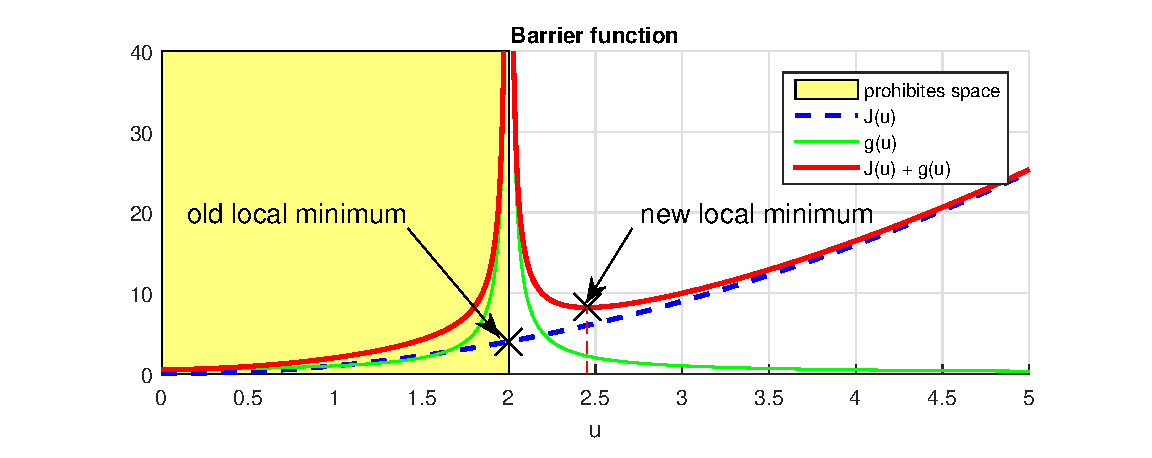
\includegraphics[width=1\textwidth]{fig/barrier_function2.eps}
\caption{Barrier function with one variable}
\label{fig:barrier_function}
\end{figure}

The Fig. \ref{fig:barrier_function} shows, how the barrier method works in one dimension. It moves the location of the strictly feasible local minimum away from the prohibited space to a a new local minimum. This is the desired property, because the strictly feasible solution can result in a bad behavior as mentioned in the beginning of this section. 

\begin{figure}[h]
\centering
\includegraphics[width=1\textwidth]{fig/LQCP2D.png}
\caption{The final optimization function with two variables}
\label{fig:barrier_function_3D}
\end{figure}

The Fig. \ref{fig:barrier_function_3D} shows the function $\macJ + \macg$ with the 2 dimensional domain. The real optimizing function is in very high dimension and can not be graphed. Principal component analysis (PCA), which is an algorithm for reducing space dimensions by projecting objects to a created basis can not be used, because it will highly deform the space.

\subsection{Gradient descent}
The optimization problem will be solved with slightly modified standard gradient descent. This is a very used algorithm for optimizing functions. It has two big requirements. One is, that the function must be differentiable. This has been satisfied by choosing quadratic function as the objective function and hyperbola as the barrier function. The second requirement is, that the function must be convex for Using the barrier method, instead of the function $\macJ$, the gradient descent optimizes the function $\macf = \macJ + \macg$ where $\macg$ is the barrier function from the Eq. (\ref{eq:barrier_function}). 
It is an iterative method, where in each iteration a point $\uvec$ is moved in the negative direction of the gradient of the function $f(\uvec)$. This means, that 

\begin{equation}
\label{eq:gradient_descend}
\uvec_{[t+1]} = \uvec_{t} - k_d \nabla \macf,
\end{equation}
where $\uvec_{[t]}$ is the $\uvec$ at the $t$-th iteration. The size of the gradient step at $i$-th iteration is $k_d \nabla \macf$.  This algorithm runs for a certain number of steps until the final $\uvec$ is used as the result. For using this algorithm, the gradient $\nabla \macf$ is needed to be computed as

\begin{equation}
\begin{split}
\nabla \macf &= \nabla \macJ + \nabla \macg\\
\nabla\macJ &= \textbf{\^H}\uvec + \textbf{\^c}\\
\nabla \macg &= k_g\sum_{i = 1}^N
\frac{\macoi.^2sig(\macoi\cdot\uvec+b_i)}
{|\macoi|\cdot(\macoi \cdot \uvec + b_i)},
\end{split}
\end{equation}
where $\macoi$ is the $i$-th line of the matrix $\textbf{A}_c$ and $b_i$ is the $i$-th member of the column matrix $\textbf{B}_c$. The notation $\macoi.^2$ represents a line vector as the diagonal of the $\macoi^T \cdot \macoi$. 

\subsection{Feasibility algorithm}
Now, that we have the $\nabla \macf$, we have to find the initial search point $\uvec_{[0]}$. Because the function $\macf$ is convex only on the feasible domain, the $\uvec_{[0]}$ has to lie there. To find a feasible $\uvec$ is not as simple task, as it looks. Especially if the UAV flies among many obstacle with higher velocity. A zero vector means flying in the initial direction and back thrust is not robust and could not work. An algorithm for finding a feasible $\uvec$ has been developed --- chci napsat, ye jsem ho vztvoril ja---, that has been named a feasibility algorithm. While developing this algorithm, a useful feature had been required. This algorithm takes a $\uvec$, that may or may not be feasible. It then finds a feasible alternative of the point, that is very close to the given one. It will be very useful for the speed and accuracy of the whole MPC, that will be discussed later. The iterative algorithm inputs are matrices $\textbf{A}_c$, $\textbf{A}_c$ and a $\uvec_0$. The algorithm can be formulated in the following steps:

\begin{enumerate}
\item Find the first constraint $\macoi \cdot \uvec_{[t]} \leq b_i$, that is violated. If such a constraint does not exist, successfully terminate the algorithm and return the $\uvec_{[t]}$.

\item Count the distance $d$ from the constraint $i$ and compute the normalized gradient $dg = \frac{\nabla \macg}{|\nabla \macg|}$.

\item Move the search point along the gradient such as $\uvec_{[t+1]} = \uvec_{[t]} + k_f \cdot d \cdot dg$ and continue to step 1.
\end{enumerate}

The constant $k_f$ should be between 1 and 2. If the $k_f$ is 1, the $u_{[t+1]}$ ends exactly on the constraint. This is not very good, because our function $\macg$ is not defined there. If the constant $k_f$ is higher than 2, the algorithm could oscillate, especially between 2 parallel constraints. From experiments, a constant $k_f = 1.5$ has been chosen and works well.

\begin{figure}[ht]
\includegraphics[width=1\textwidth]{fig/feasibility_paint.eps}
\caption{Feasibility algorithm.}
\label{fig:feasibility_algorithm}
\end{figure}


The Fig. \ref{fig:feasibility_algorithm} shows, how the algorithm can correct a $\uvec$, that is not feasible into a feasible one with a position very close to the initial one. 

When the algorithm for tracking trajectory starts, the UAV has no velocity, so the gradient descent algorithm can use the initial search point $\uvec_{[0]}$ as a zero vector. It means, that it will stay at one place, so there is no predicted collision. The MPC loop runs very fast and if every time a new gradient descend is initialized with a random $\uvec_{[0]}$, it would take a long time to come anywhere to the local minimum. The knowledge, that the UAV moves relatively slow compared with the MPC loop, can be very useful, because the function $\macf$ is very similar in the next step. A final prediction from previous MPC step can be used as an initial search point. This incredibly increases the speed and accuracy of the gradient descend algorithm. Of course, this could not have been done without the feasibility algorithm. A final $\uvec$ from previous MPC step can be feasible no more with a different UAV position and velocity. This is, where the required feature of the feasibility algorithm comes handy. It moves the previous $\uvec$ to a new location, that is still very close to the previous $\uvec$, so very close to the local minimum. 

There can be a situation, where a feasible solution does not exist. In this case, the loop would run infinitely. This can be achieved especially, if the sensory noise is too high that a distance to an obstacle is evaluated closer, then the $R_{UAV} + r_obs$. With this initial condition there is usually no solution as described in the section \ref{sec:safe_margin}. To prevent the UAV to freeze, a counter needs to be added to terminate the feasibility algorithm after running too long.

\subsection{Implementation of the gradient descend}
\label{sec:implementation_of_the_gradient_descend}
The gradient descend is implemented by the equation \ref{eq:gradient_descend}. The only difference is, that in every iteration, every $\uvec_{[t]}$ is checked for feasibility by applying the feasibility algorithm. The reason to do this is, that the gradient step can be too big and after shifting the search point, it can end up outside the feasible domain. If the gradient step constant $k_d$ was set too small, it would take longer time to converge to the local minimum. The $k_d = 150$ based on simulations and experiments.

A simulation has been run for no barrier function using only the $\nabla \macJ$ and the feasibility algorithm and still providing fairly good results. This approach has not been used in later simulations or experiments.

Choosing the total number of iterations of the gradient algorithm generally depends on the requirements of accuracy vs speed. Experimentally has been observed, that a small number of total iterations can be helpful by providing a low pass filter in situations with high sensory noise. Experiments have shown, that 100 iterations is a good compromise between the accuracy and the speed.

\section{Move Blocking}

The whole MPC algorithm is very demanding on computational time and memory. This can result in a very slow frequency of the MPC controller. A matrix multiplication of a $n$ by $m$ matrix and a column vector of the length $m$ has the computational complexity $O(nm)$. For example the matrix $\textbf{\^B}$ is the size of $6T$ by $2T$ and the vector $\uvec$ is the length of $2T$. This makes the computational complexity $O(12T^2)$. When considering, that the system model is created for $dt = 1/70s$, for prediction of 2 seconds for a simple matrix multiplication, processor would have to do at least $12 \cdot  140^2 = 235 200$ operations. With the size of 4 bytes for one float, the matrix $\textbf{\^B}$ would take almost 1\jed{MB} of memory. This is not that much for PC simulation, but it is a lot for the custom board flying on the UAV with only 192 kB RAM, 2 MB of ROM and 168 MHz processor with one instruction for float multiplication. 

\subsection{Move blocking implementation}
The computation complexity can be greatly reduced by reducing the $T$, which is the total number of future predictions. The discretization of the prediction is very soft, meaning, that the $\Delta t$ is very small. With the maximum speed this is a distance 0.5\jed{mm} between predicted positions. There is no reason to predict position 70 times a second. The input actions tend to take form of a continuous function. One solution would be to change the system's $\Delta t$, but there is a better solution. Move blocking algorithm allows us to choose exactly which time steps will be used. This allows only small number of variables to cover long prediction horizon. The algorithm will generate constant input action between those predicted as shown in Fig. \ref{fig:move_blocking}. Let's introduce a matrix $\textbf{U}$ of the height $2T$ and width $2T_n$, where $T_n$ is the new number of predicted states. This matrix determines, which time steps will be used.

\begin{figure}[h]
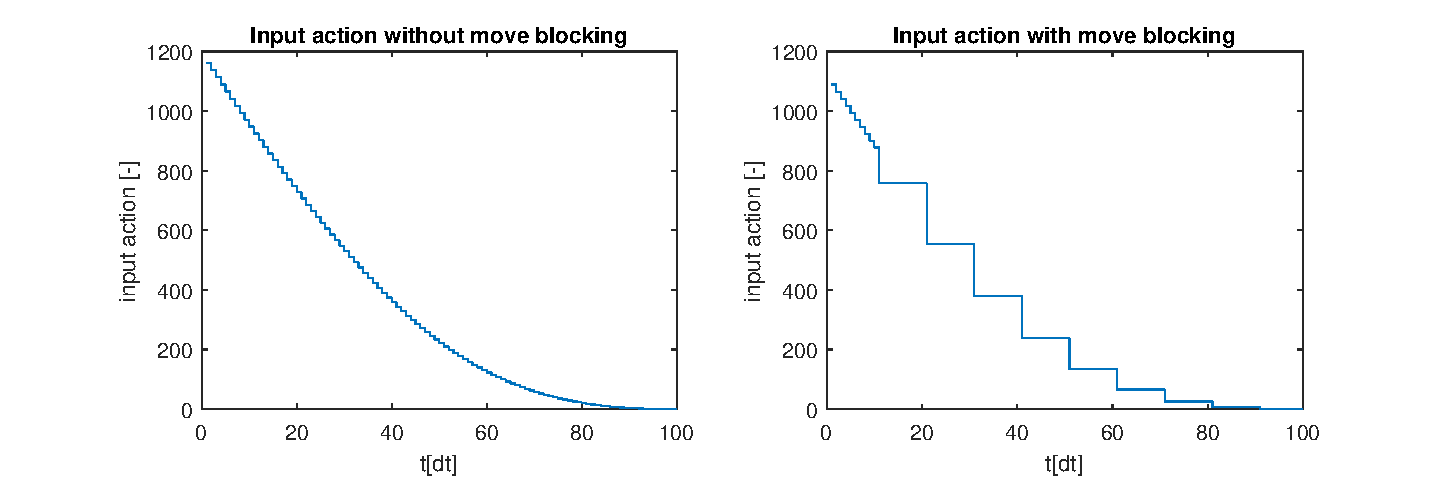
\includegraphics[width=1\textwidth]{fig/move_blocking_u.eps}
\caption{Move blocking algorithm in one axis}
\label{fig:move_blocking}
\end{figure}

\begin{equation}
\uvec = \underbrace{\begin{bmatrix}
\begin{bmatrix}
1\\
\vdots\\
1
\end{bmatrix} & \textbf{0} & \hdots & \textbf{0} \\
\textbf{0} & \begin{bmatrix}
1\\
\vdots\\
1
\end{bmatrix} & \hdots & \textbf{0}\\
\vdots & \vdots & \ddots & \vdots \\
\textbf{0} & \textbf{0} & \hdots & \begin{bmatrix}
1\\
\vdots\\
1
\end{bmatrix}
\end{bmatrix}}_{\textbf{U}}\urvec, \;\;
\urvec = \begin{bmatrix}
\textbf{u}_{[t_1]} \\
\textbf{u}_{[t_2]} \\
\vdots \\
\textbf{u}_{[T_r]}
\end{bmatrix},
\label{eq:moveblocking_example}
\end{equation}
$\urvec$ is the reduced column vector of the length $2T_r$. Its members are time predictions at certain times $t_1, t_2, ..., T_r$. All matrices introduced in MPC must be reduced. The process is quite complicated and will not be described step by step. 

In the figure \ref{fig:move_blocking} have been used prediction times $1, 2, ..., 9, 10, 20, 30, ..., 100$. The number of the prediction times is $T_r$. Using this particular vector, the $T_r$ is 19 instead of $T$ as 100. The acceleration of matrix multiplication can be computed as $(T/T_r)^2 = 27.7$. This means $27.7$ times faster. The move blocking algorithm also creates the same memory savings with some matrices. This is a crucial improvement of the MPC algorithm, allowing to cover a longer prediction horizon without having too big matrices.

The penalization matrices $\textbf{Q}$ and $\textbf{P}$ need to be edited a little bit differently. Without move blocking, all predicted positions and inputs are penalized evenly. If now the predicted inputs represents inputs of different length, the penalization must be set accordingly. The main diagonal has to have its members individually multiplied by the corresponding constant of the number of the representing time steps. 


\section{Simulations and Hardware}
\begin{figure}[h]
\centering
\begin{subfigure}{.48\textwidth}
  \centering
  \includegraphics[width=1\linewidth]{fig/dron_up}
\end{subfigure}%
\begin{subfigure}{0.48\textwidth}
  \centering
  \includegraphics[width=1\linewidth]{fig/dron_strana}
  \label{fig:blob}
\end{subfigure}
\captionof{figure}{UAV body}
\end{figure}

Developing the collision avoidance system just on the paper and then programming it directly to the UAV's on-board computer is a very naive approach that very likely would not work. To minimize the probability of an expensive crash happening, the algorithm should be tested as much as possible. 


\subsection{Simulation}

During the development of the MPC, all steps were being tested by Matlab simulations. This program is good for these purposes, because it is optimized for matrix multiplication, which is the core of he MPC computing. The matlab simulation consists of two separate modules: the Environment module and the UAV module. 

\subsubsection{The Environment module}

The Environment module simulates the flight. This simulates the physical world and the sensors of the UAV. It is initialized by the obstacles positions, the UAV's initial condition and desired trajectory. It takes care of the UAV's dynamics and simulates the flight. The main program runs in a loop. It receives the computed input actions from the UAV module and computes the UAV's movement. Then it updates the relative obstacles positions, the absolute UAV position and the velocity and the desired trajectory. It then gives this information as an input to the UAV module. 
This module also sets the parameters for the UAV module, such as penalization of the position errors $k_q$ and the input $k_p$, the indexes of the move blocking time predictions and gradient descend iterations and step size. This makes it easier to tune the overall constants.

It has also the ability to visualize the UAV, obstacles, the desired trajectory, the predicted trajectory and the convex feasible space. This graph updates with the loop, so it simulates the whole flight. 

\begin{figure}[h]
\centering
\includegraphics[width=1\linewidth]{fig/phantom.jpg}
\caption{Simulation visualization.}
\label{fig:phantom}
\end{figure}

\subsubsection{The UAV module}

The second module simulates the the MPC controller on UAV's on-board computer. It has the ability to compute the input actions based on the information received from the Environment module. It consists of two parts. 

First, the MPC problem definition, which creates the constraining matrices $\textbf{A}_c$, $\textbf{B}_c$ from the information about the initial condition and obstacles positions. Only the objective function matrix $\maccr$ is created, because the $\macHr$ is a constant and can be stored in memory.

Second, the LCQP solver. This solver has been written by the method described in the Sec. \ref{sec:implementation_of_the_gradient_descend}. Its inputs are the gradient step size, the total number of iterations and the problem defining matrices, which are identical to the function quadprog from the optimization toolbox. It returns slightly different result, because it returns on purpose not strictly feasible solution. 



\subsection{UAV custom board}
\label{sec:custom_board}
The UAV custom board \cite{tomas} as shown in the Fig. \ref{fig:Cutom_board}, is a computer with very limited computational power compared to matlab. This board has been designed \cite{tomas} especially for MPC control and communication. This board is whole programmed in the language C. It has two computational units: xMega and STM. For debugging and data logging is a socket for XBee and logging data to micro SD card. This board sticks to the philosophy of distributed computing.

\begin{figure}[h]
\label{fig:Cutom_board}
\centering

\begin{subfigure}[b]{0.515\textwidth}
	\begin{tikzpicture}
		\node[anchor=south west,inner sep=0] (a) at (0,0) {\includegraphics[width=\textwidth]{fig/board1.jpg}};
		\begin{scope}[x={(a.south east)},y={(a.north west)}]

				%\draw[help lines,xstep=.1,ystep=.1] (0,0) grid (1,1);	
		
        \draw[white,ultra thick,rounded corners] (0.55,0.50) rectangle (0.7,0.7);
        \draw (0.58,0.655) node [text=white] {\textbf{1}};
        
        \draw[white,ultra thick,rounded corners] (0.23,0.17) rectangle (0.345,0.3);
        \draw (0.26,0.26) node [text=white] {\textbf{2}};
        
        \draw[white,ultra thick,rounded corners] (0.5,0.06) rectangle (0.72,0.37);
        \draw (0.55,0.25) node [text=white] {\textbf{3}};
        
        \draw[white,ultra thick,rounded corners] (0.09,0.69) rectangle (0.39,0.78);
        \draw (0.12,0.73) node [text=white] {\textbf{4}};
        
        \draw[white,ultra thick,rounded corners] (0.09,0.34) rectangle (0.39,0.42);
        \draw (0.12,0.38) node [text=white] {\textbf{4}};
    \end{scope}
	\end{tikzpicture}
	\caption{board's top}
	\label{fig:board_top}
\end{subfigure}%
\begin{subfigure}[b]{0.485\textwidth}
	\begin{tikzpicture}
		\node[anchor=south west,inner sep=0] (a) at (0,0) {\includegraphics[width=\textwidth]{fig/board2.jpg}};
		\begin{scope}[x={(a.south east)},y={(a.north west)}]

				%\draw[help lines,xstep=.1,ystep=.1] (0,0) grid (1,1);	
		
        \draw[white,ultra thick,rounded corners] (0.71,0.50) rectangle (0.79,0.59);
        \draw (0.75,0.545) node [text=white] {\textbf{5}};
    \end{scope}
	\end{tikzpicture}
	\caption{board's bottom}
	\label{fig:board_bottom}
\end{subfigure}

\caption{Custom control board v.2, key components are placed at follows: 1 -- xMega, 2 -- STM, 3~--~switching power supply, 4 -- socket for XBee, 5 -- data logging MCU.}
\end{figure}

The xMega is a slow computational unit. It has 8-bit architecture with 32 MHz clock and 8 kB SRAM. It is mainly handling the communication between sensors and STM. The communication between peripherals goes through 7 UART ports. Sensors or a computer can be connected. With the help of the program Putty, a simple messages can be exchanged between the computer and the board. Most of the protocols have been already designed, but minor adjustments had to be done to fit the exact requirements of collision avoidance. For example the communication between the xMega and STM had to be extended to transfer information about obstacle positions. The xMega also stores the desired trajectory or the location of the desired position(setpoint) and it sends this data to the STM. 

The STM is a powerful 32-bit unit with 168 MHz clock and 192 kB of RAM and 2\jed{MB} ROM. This runs three tasks: 

\begin{itemize}
\item CommTask is responsible for communicating between the xMega and STM.

\item KalmanTask is the state estimator task responsible for estimating positions, velocity, acceleration and input error based on information from the px4flow sensor and the inputs. When it computes the state, it sends it to the MPCTask.

\item MPCTask is the task, that computes the MPC controller. The MPC is triggered by the KalmanTask, if the previous iteration has finished. This means, that if the MPC  runs slower, than 70 Hz, it does not cause big problems, because the input actions are held, until they are replaced by a new ones. This mechanism allows tuning between the speed and accuracy of the MPC, because there i	s no need to regulate the UAV with 70 Hz.
\end{itemize}

Each task uses a third of the CPU time and 16\jed{kB} RAM. Because of very limited computational power, the MPCtask has to be programmed very efficiently.

%\begin{comment}
\begin{figure}[ht]
\centering
\includegraphics[width=1\textwidth]{fig/STM_xMega.eps}
\caption{Block diagram of information 
ow between tasks of xMega and STM MCUs.}
\label{fig:feasibility_algorithm}
\end{figure}

\subsection{Obstacles detection}
A system WhyCon\cite{whycon_icar}\cite{whycon_jint} is used for obstacle detection. It uses 3 Mobius Actioncam cameras, two pointing to the sides and one forwards. This allows obstacle detection at 270$^\circ$. Each camera has the capability of recording in the resolution 1920x1080, but for faster performance the video is shoot in 1280x720 and processed 640x480. The system is capable of precise detecting of multiple circular markers shown in Fig. \ref{fig:blob}. The 3-axis positions of these markers are then sent by UART to the custom board, where the xMega receives the information. The image processing runs in a loop on a computational unit NVIDIA Jetson TK1.

\subsection{MPC hardware implementation}

The exact algorithm, as written in matlab, has been rewritten to the C code. This has been the most time demanding part of this thesis. The programmed code uses a CMatrixLib library, that allows simple matrix and vector operations. This library has been extended by more functions for the purposes of this thesis. Because the RAM is very limited, the matrices have to be divided into constant matrices, that are stored in ROM, and the changing matrices, which have allocated memory in RAM.

The constant matrices depend only on the system model and move blocking algorithm. These matrices are: $\textbf{\^A}_x$, $\textbf{\^A}_y$, $\textbf{\^B}_x$, $\textbf{\^B}_y$, $(\textbf{\^Q}\textbf{\^B})^T, \textbf{\^A}$ and $\textbf{\^H}$. They had been adapted by the move blocking algorithm, generated in matlab and stored in the ROM memory of the STM unit. 

The UAV's max speed has been set to 0.35\jed{ms^{-1}}. This is enforced by editing the desired trajectory. If the trajectory doesn't violate the maximum speed, it is used unchanged. In the other case, the desired positions are moved closer to the UAV. If given only setpoint, the desired trajectory is created as a straight line with the maximum speed. 

The input action can not be infinite and some method of constraint has to be applied. Applying the constraints in the MPC control slows the algorithm down. A saturation of the output has been used instead.


\subsection{Hardware in the loop}
This is a method of testing embedded hardware. The custom board is connected to a computer instead of UAV's body. The board's inputs are provided by the computer and outputs are sent back. The board is in the same situation, as if it would be flying.  This has been simulated in two experiments. 

The first one was connecting the board to the computer using the putty terminal. The inputs have been sent through the terminal and outputs were received. These outputs were compared with the matlab simulations, to check if they match. The UAV has been tested in various situations, such as different initial conditions, desired trajectories and obstacle positions. This allowed to test and debug the various segments of the code, as well as the MPC algorithm as whole. This method also allowed to test xMega as well as STM. After successfully finishing this testing, it was sure, that the implemented algorithm behaves exactly in the same way as the simulation.

The second experiment was connecting the board to the UAV, without the ability of controlling the motors. It received inputs from the UAV's sensors, such as velocity and obstacle positions. The board was connected to matlab using wireless Xbee. The Xbee communication protocol has been extended for the important information to be transferred. A matlab visualization allowed to see the predicted trajectory in real time without the need to be connected to the UAV with a cable. This allowed testing the algorithm in real situations without worrying of damaging the UAV. It also allowed testing communication with the on-board sensors. The frequency of the MPC loop has been measured close to 20\jed{Hz}. This is an sufficient regulator frequency.

After testing in various situations and behaving correctly, it was time to do a real flight experiment.

\section{Experiments}

\begin{figure}[h]
\centering
\includegraphics[width=1\textwidth]{fig/experiment_photo}
\caption{Photo of the obstacle avoidance experiment.}
\label{fig:move_blocking}
\centering
\end{figure}

The implemented MPC controller has been verified by a real world experiments. Simulations, that have been done, differ from the real world experiments mainly by the absence of sensory noise. Because of the construction of the UAV with 4 propellers on sides, most collisions can be dangerous not only for the UAV, but for the operator as well. That is the reason, why the operator has to have the access to take over the control any time during these experiments. During the described experiment this possibility has not been used and the presented data are solely while the MPC was in control.

\subsection{Stabilization}
The first experiment was to test the stability and settle time of the MPC. The position setpoint was set to the origin of the world coordinate system. The task for the UAV was to track this setpoint while the UAV was physically pushed by the operator. This tested reactions of the controller to an outside disturbances.


\begin{figure}[h]
\centering
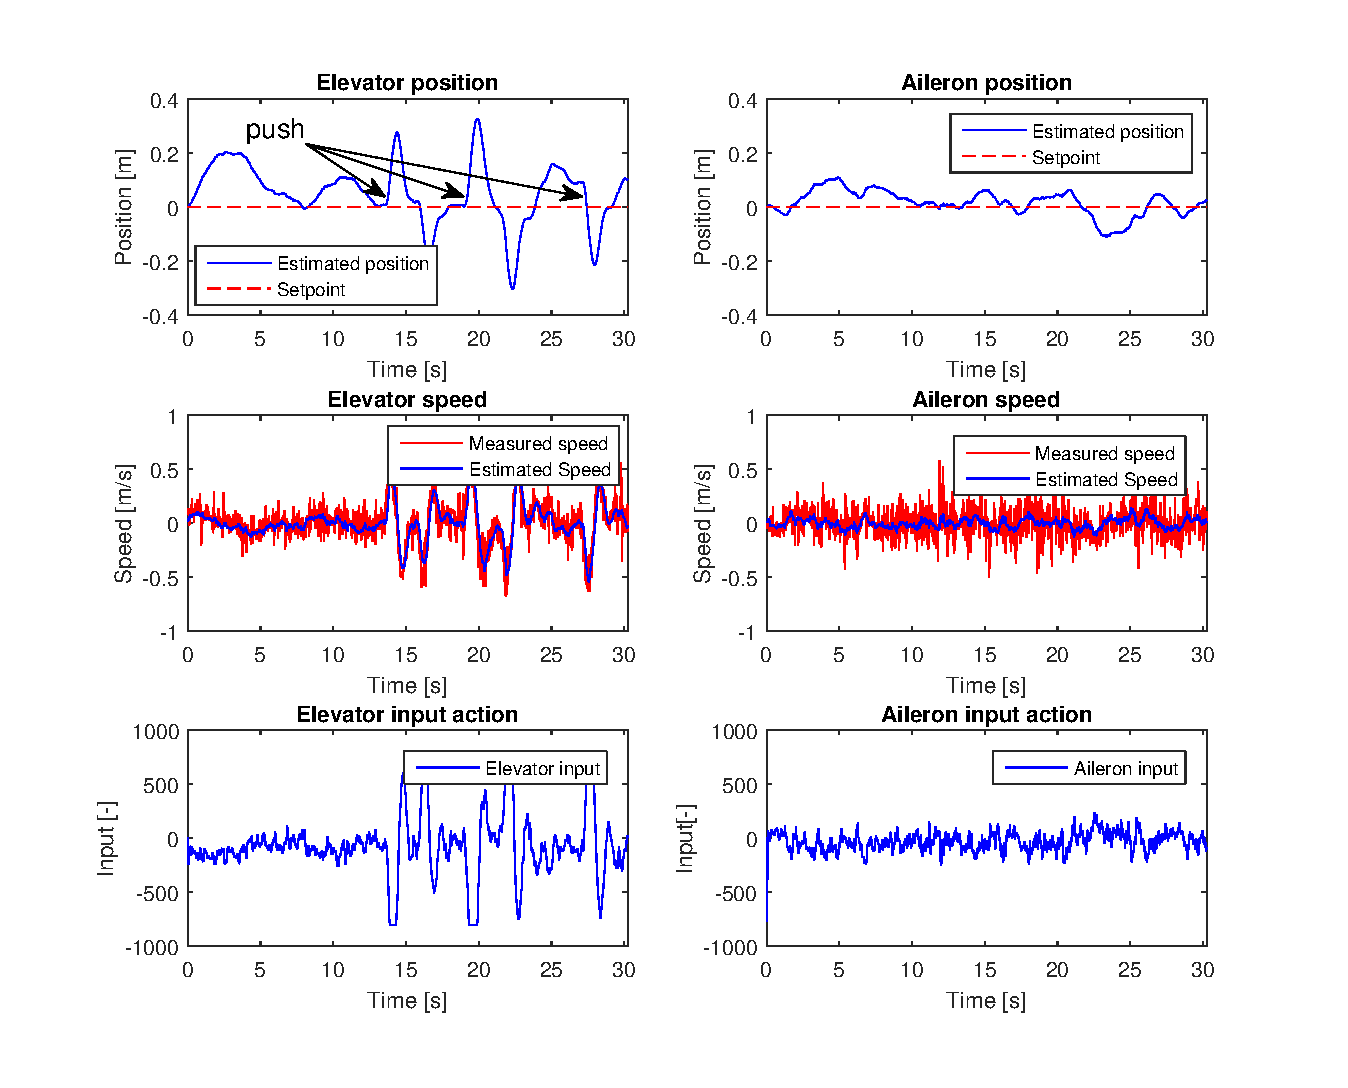
\includegraphics[width=1\textwidth]{fig/balancing.eps}
\caption{Data from the stabilization experiment}
\label{fig:stabilization}
\end{figure}

The Fig. \ref{fig:stabilization} shows the position, speed and input action during the stabilization experiment. During the experiment, the UAV has been three times pushed in the positive direction of the elevator axis. The UAV returned then to the original position. The aileron position stayed away from the setpoint within 11\jed{cm}, which is a good performance considering the size of the UAV's body. At the elevator axis it is 20\jed{cm} if not considering the disturbances.

\subsection{Obstacle avoidance}
The obstacle avoidance system has been tested. The obstacle was represented by a blob - recognizable pattern by the camera. This was especially risky experiment, because the UAV had to get close to the obstacle. The maximum speed was set to 0.2\jed{ms^{-1}} for the operator to have enough time to take control of the UAV in case incorrect behavior. The UAV was given a setpoint 4\jed{m} in the front. The obstacle was in the middle between the UAV's initial position and the setpoint and did not move. The obstacle was given a predefined diameter of 0.5\jed{m}. The trajectory was being created on-board. This way the algorithm of creating trajectory was tested as well. The task was to avoid the obstacle and arrive to the setpoint position.

\begin{figure}[h]
\centering
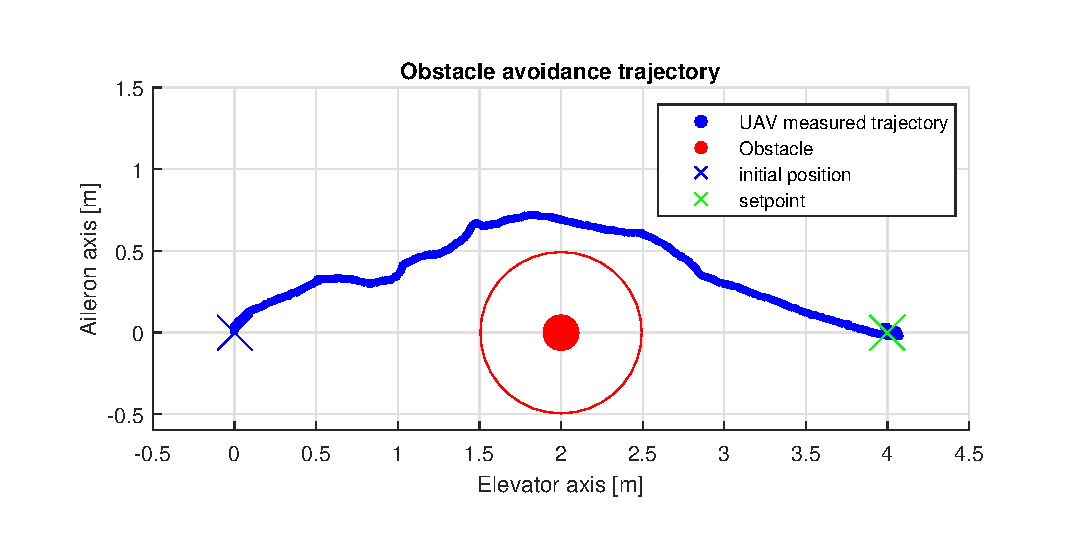
\includegraphics[width=1\textwidth]{fig/avoidance_experiment.eps}
\caption{Obstacle avoidance experiment}
\label{fig:avoidance_experiment}
\end{figure}

The fig. \ref{fig:avoidance_experiment} shows the UAV's obstacle avoidance trajectory. Around the obstacle is a red circle of 0.5\jed{m}, which is the minimal distance allowed from the obstacle. The figure also shows, that there is a safe distance from the obstacle, which was enforced by the barrier function. The UAV also finishes on the setpoint and stabilizes there.

\section{Conclusion}
In this thesis a Model predictive controller for UAV has been developed. It is capable of trajectory or setpoint tracking and obstacle avoidance. The MPC algorithm and linearly constrained quadratic programming solver has been designed and tested by matlab simulations. The solution was then implemented on embedded hardware and tested again. Real world experiments have been successfully conducted. The UAV was capable of trajectory tracking while detecting and avoiding an obstacle. The entire assignment of this thesis has been successfully fulfilled.

\subsection{Future work}
Although simulations and experiments have been successfully executed, there is still a room for future improvements. The greatest limitation of the introduced algorithm is keeping the convexity of the mathematical optimization. If this condition was lost, the optimization problem would have local minimums, but the designed prediction space could be much more complex, allowing the UAV to work with more complicated obstacles. This would allow UAV to fly faster and safer.





\end{document}